\documentclass[11pt,a4paper]{article}
\usepackage[a4paper,top=19mm,bottom=20mm,left=22mm,right=22mm,headsep=7mm]{geometry}
\usepackage{fontspec}
\IfFontExistsTF{Times New Roman}
  {\setmainfont{Times New Roman}}
  {\setmainfont{TeX Gyre Termes}}
\IfFontExistsTF{Arial}
  {\setsansfont{Arial}}
  {\setsansfont{TeX Gyre Heros}}
\usepackage{unicode-math}
\IfFontExistsTF{STIX Two Math}
  {\setmathfont{STIX Two Math}}
  {\setmathfont{TeX Gyre Termes Math}}
\usepackage[main=russian,english]{babel}
\usepackage{microtype}
\usepackage{amsmath,mathtools}
\usepackage{graphicx}
\usepackage{booktabs,tabularx,array}
\usepackage{siunitx}
\usepackage{caption}
\usepackage{tikz}
\usetikzlibrary{arrows.meta,positioning,calc}
\usepackage{xcolor}
\usepackage{hyperref}
\usepackage{fancyhdr}
\usepackage{titlesec}
\usepackage{setspace}
\usepackage{enumitem}
\usepackage{float}
\usepackage{placeins}

\definecolor{airiblue}{HTML}{235F9C}
\definecolor{airiteal}{HTML}{0F857C}
\definecolor{airired}{HTML}{B84848}
\definecolor{airigray}{HTML}{65727C}

\hypersetup{
  colorlinks=true,
  linkcolor=black,
  citecolor=airiblue,
  urlcolor=airiblue,
  pdftitle={Последовательное прогнозирование движения клеток с локальным переносом невязок},
  pdfauthor={Дмитрий Станиславчук-Абовский; Андрей П. Захаров}
}
\sisetup{detect-all=true}
\setstretch{1.08}
\setlength{\parindent}{1.25em}
\setlength{\parskip}{0pt}
\renewcommand{\arraystretch}{1.04}
\newcolumntype{Y}{>{\raggedright\arraybackslash}X}
\newcolumntype{L}[1]{>{\raggedright\arraybackslash}p{#1}}
\setlength{\emergencystretch}{2em}
\setlength{\textfloatsep}{9pt plus 2pt minus 2pt}
\setlength{\floatsep}{8pt plus 2pt minus 2pt}
\setlength{\intextsep}{8pt plus 2pt minus 2pt}
\captionsetup{
  font=small,
  labelfont=bf,
  labelsep=period,
  justification=justified,
  singlelinecheck=false,
  skip=4pt
}
\renewcommand{\figurename}{Рисунок}
\renewcommand{\tablename}{Таблица}
\renewcommand{\refname}{Литература}
\titleformat{\section}{\large\bfseries}{\thesection.}{0.6em}{}
\titleformat{\subsection}{\normalsize\bfseries}{\thesubsection.}{0.6em}{}
\titlespacing*{\section}{0pt}{14pt}{5pt}
\titlespacing*{\subsection}{0pt}{10pt}{3pt}
\pagestyle{fancy}
\fancyhf{}
\fancyhead[L]{\footnotesize Последовательное прогнозирование движения клеток}
\fancyhead[R]{\footnotesize Исследовательская версия}
\fancyfoot[C]{\thepage}
\renewcommand{\headrulewidth}{0.35pt}
\renewcommand{\footrulewidth}{0pt}
\setcounter{secnumdepth}{2}
\sloppy
\begin{document}

\begin{center}
{\LARGE\bfseries Последовательное прогнозирование движения клеток с локальным переносом невязок\par}
\vspace{5mm}
{\normalsize Дмитрий Станиславчук-Абовский, Андрей П. Захаров\par}
\vspace{2mm}
{\small 1 августа 2026 г.\par}
\end{center}
\vspace{4mm}

\noindent\textbf{Аннотация.}\enspace Краткосрочное движение отдельной клетки в плотной ткани определяется собственной динамической памятью, коллективным состоянием окружения и ошибкой измерения, однако эти составляющие лишь частично наблюдаемы по координатам центроидов. Мы исследовали, какие сведения улучшают прогноз следующего смещения без будущих наблюдений, и построили последовательную архитектуру, в которой прогноз каждого перехода фиксируется до появления нового кадра. Базовый модуль использует историю трека и скорости; рекуррентная модель задает распределение Стьюдента и обновляет состояние по ошибке завершенного перехода; ограниченный многомасштабный граф переносит в следующий прогноз измеренные невязки соседей. В шести внешних циклах MDCK Bulk режим ближайшего шага достиг RMSE 3,474 пикселя и $R^2=0{,}508$ на h1. Отдельный накопительный режим достиг RMSE 5,501 и $R^2=0{,}938$ на h6, уменьшив среднюю по фильмам ошибку на 29,8\% относительно модели без локального переноса и на 17,4\% относительно постоянной скорости. В замороженной проверке на семи фильмах MDCK Bulk 10--16 накопительный режим достиг h6 RMSE 4,820; улучшение 25,82\% наблюдалось в 7/7 фильмах. Знаково ограниченный E(2)-эквивариантный закон с общими для двух координат коэффициентами воспроизвел 96,5\% выигрыша плотной поправки на разработческих фильмах и, без настройки на фильмах 10--16, достиг h6 RMSE 4,842, $R^2=0{,}952$ и выигрыша 25,46\% в 7/7 фильмах; неправильные время и клеточная идентичность разрушали эффект. На независимом наборе из 22 островков MDCK потенциальный полевой закон уменьшил ошибку полного шестишагового развертывания на 6,30\% в 22/22 внешних циклах. Его конечное обновление уменьшало подобранный функционал во всех 398 проверенных кадрах, но наблюдаемая ткань делала это лишь в 51,3\% кадров против 49,2\% при временной перестановке. Поэтому функционал является математическим свойством модели, а не установленной физической энергией; измеренная тяга и напряжение также не прошли причинные контроли. Внешняя по фильму калибровка дала радиальное покрытие 89,7\% для номинального 90\%-интервала h6. Метод имеет наименьшую h6 RMSE среди завершенных согласованных базовых методов этой работы в зафиксированном последовательном протоколе LaChance; преимущество h1 и глобальное превосходство для всех задач прогнозирования траекторий не заявляются.

\vspace{2mm}
\noindent\textbf{Ключевые слова.}\enspace Коллективная миграция клеток, последовательное прогнозирование, фильтрация состояния, локальное взаимодействие, граф соседства, неопределенность.

\vspace{2mm}
\noindent\textbf{Краткое авторское резюме.}\enspace
Клетки в плотном слое движутся не независимо: их шаги связаны с историей самой клетки и с изменениями ближайшего окружения. Однако по одному текущему кадру обычно невозможно надежно определить, куда именно сместится отдельная клетка. Мы показали, что полезную информацию можно извлекать последовательно. Сначала модель предсказывает следующий шаг и сохраняет этот прогноз. После появления нового кадра она измеряет собственную ошибку и ошибки соседних клеток, а затем использует только уже завершенные движения для следующего прогноза. Такой порядок исключает просмотр будущего и соответствует работе с поступающим потоком микроскопических изображений. На нескольких типах клеток локальный перенос недавно измеренных ошибок заметно уменьшал накопление погрешности на последовательности из шести кадров. Сигнал ослабевал при увеличении расстояния и разрушался, если подменить время или клеточную идентичность. Разреженный вариант использовал лишь часть возможных связей между клетками и почти линейно масштабировался с размером поля. Полученная поправка не является измеренной силой: она объединяет неописанное движение ткани, биологическую изменчивость и ошибки наблюдения. Работа предлагает проверяемый способ использовать эту коллективную составляющую, не приписывая ей заранее заданный физический закон.

\section{Введение}
Коллективная миграция участвует в морфогенезе, заживлении тканей, ангиогенезе и опухолевой инвазии \cite{ref1,ref2,ref3,ref4}. Движение наблюдаемой клетки возникает из сочетания собственной поляризации, межклеточных контактов, тяги к субстрату, пространственного распределения напряжений, геометрии границы и перестройки цитоскелета. Эти процессы активны, анизотропны и обладают памятью. Поэтому одинаковая конфигурация центроидов может предшествовать различным направлениям движения, а описание статистически типичного окружения не обязательно определяет следующий индивидуальный шаг.

Временная микроскопия дает координатные треки, но координата является неполной проекцией состояния клетки. В наблюдаемом смещении смешиваются биологическое движение, коллективное возмущение, неточность центроида и возможная ошибка клеточной идентичности. Это ограничивает как механическую интерпретацию, так и обычный многокадровый прогноз. В наших опытах генеративные модели строили широкое облако будущих траекторий и уменьшали минимальную ошибку среди 32 кандидатов приблизительно на 5-10\%, однако выбрать правильного кандидата до наблюдения цели не удавалось. Следовательно, геометрическое покрытие будущего и идентификация реализующегося режима являются разными задачами.

Большая часть методов многорежимного прогнозирования траекторий, включая AgentFormer, MTR, QCNet и EigenTrajectory, использует устойчивую геометрию допустимых маршрутов, тип агента или выраженный контекст сцены \cite{ref8,ref9,ref10,ref11,ref12,ref13}. В клеточном слое заранее размеченной карты маршрутов нет, а локальное состояние может быть скрыто от одной модальности. Графовые сети способны описывать обмен сообщениями, но дополнительная глубина не создает отсутствующий во входах прогностический сигнал. Аналогично, морфологическое или механическое состояние может быть биологически содержательным и одновременно недостаточно связанным со следующим остаточным смещением в конкретном экспериментальном протоколе.

Работы по клеточному движению обычно решают более узкие задачи: классифицируют поворот, восстанавливают усредненные правила взаимодействия или прогнозируют направление по одному изображению \cite{ref1,ref5,ref21}. Это делает прямое ранжирование с транспортными моделями некорректным без выравнивания времени выдачи прогноза и доступных наблюдений. В данной работе все численные сравнения приведены к одному последовательному протоколу: метод сначала фиксирует оценку следующего смещения, а затем получает новый кадр. Архитектуры фиксированного многокадрового прогноза обсуждаются как проверка идей, но не смешиваются с основной таблицей.

Последовательная фильтрация дает естественный способ обновлять скрытое состояние по уже состоявшейся ошибке. KalmanNet обучает аналог коэффициента Калмана для частично известной динамики, а распределение Стьюдента делает вероятностное обновление устойчивее к тяжелым хвостам \cite{ref6,ref7}. Однако индивидуальный фильтр не описывает совместную пространственную часть ошибки. С другой стороны, современные представления живых клеток учатся по временной согласованности трека, направлению времени и маскам \cite{ref16,ref17,ref18,ref19}. Их польза для прогноза требует более строгого критерия, чем распознавание внешнего вида: признаки правильной клетки и времени должны превосходить межклеточную и временную подмены. Такое разделение индивидуального состояния, качества наблюдения и локального поля определило как архитектуру, так и отрицательные контроли работы.

Другой класс работ восстанавливает интерпретируемые гидродинамические уравнения активной материи из полевых наблюдений, ограничивая библиотеку членов симметриями и проверяя характерные пространственно-временные спектры \cite{ref32}. Такой подход требует отличать обнаружение устойчивого кинематического оператора от идентификации механической силы. В клеточной ткани одновременные поля скорости, тяги и напряжения позволяют проверить это различие непосредственно \cite{ref24}: улучшение прогноза за счет производных поля еще не доказывает, что коэффициенты соответствуют измеренной механике.

Мы поэтому изменили не биологическую цель, а временную постановку. Модель предсказывает один следующий переход, затем получает уже состоявшееся наблюдение и только после этого обновляет состояние. Накопительные h2, h4 и h6 показатели образуются последовательностью таких прогнозов. Такой протокол соответствует потоковой микроскопии и позволяет использовать новую информацию без просмотра будущего. Ключевым наблюдаемым объектом становится завершенная невязка прогноза, то есть разность между состоявшимся смещением и оценкой, записанной до появления кадра. В теории фильтрации эта величина соответствует innovation residual; далее используется более естественный русский термин «невязка».

Итоговый метод далее обозначается LIT-Cell (Local Innovation Transport for Cell Motion). Работа дает три связанных результата. Во-первых, систематическая проверка статической парной физики, свободных графовых сетей, генераторов кандидатов, прямых видеоветвей и внешних механических признаков отделяет наличие биологического сигнала от его прогностической доступности до следующего кадра. Во-вторых, невязки сильного индивидуального прогноза образуют устойчивое локально коррелированное поле, которое проходит пространственный, временной и идентификационный контроль. В-третьих, компактная последовательная модель, объединяющая базовый координатный прогноз, устойчивое к выбросам вероятностное обновление и ограниченный перенос невязок, уменьшает накопительную ошибку в четырех клеточных доменах. Полный реестр проверенных и исключенных ветвей приведен в дополнительном материале.


\begin{figure}[tb]
\centering
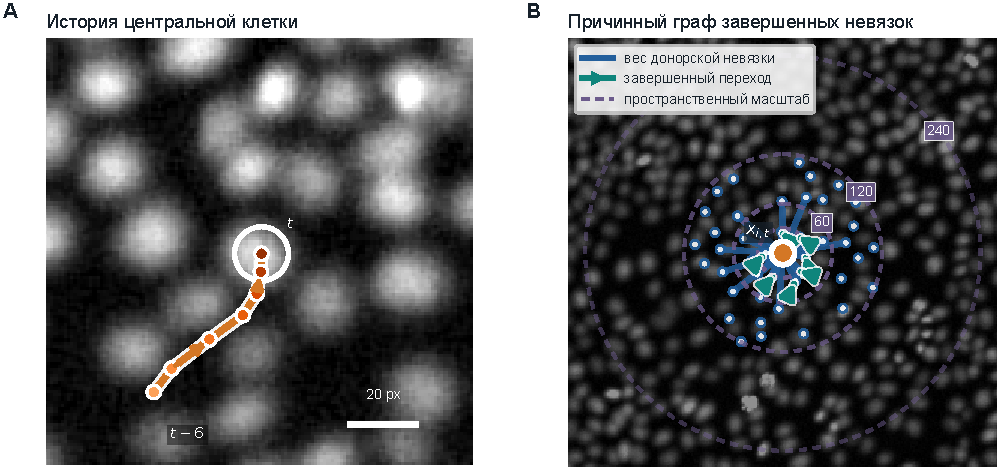
\includegraphics[width=\textwidth]{figures/fig1_real_cells_graph.pdf}
\caption{Исходные наблюдения и построение локального причинного графа. \textbf{A}, увеличенный фрагмент реального кадра MDCK Bulk. Показаны семь доступных положений центральной клетки от $t-6$ до $t$; стрелки указывают направление уже наблюденной истории, координата $t+1$ не показана. \textbf{B}, при выпуске прогноза для клетки $i$ ее положение $x_{i,t}$ связывается с положениями клеток-доноров в предыдущем кадре. Вес донора равен $w_{ij}^{(\ell)}=\exp[-\|x_{i,t}-x_{j,t-1}\|^2/(2\ell^2)]$ для $\ell\in\{30,60,120,240\}$ px; собственный трек исключается. Бирюзовые стрелки показывают завершенные переходы доноров, из которых после вычитания ранее сохраненного прогноза получаются невязки. Для читаемости нанесены 20 наиболее весомых ребер; при расчете используются все допустимые доноры внутри адаптивной опоры $R_t=4\xi_{\mathrm{train}}d_{\mathrm{nn},t}$, где $\xi_{\mathrm{train}}$ оценена только по обучающим фильмам внешнего цикла. Микроскопическое изображение служит геометрической иллюстрацией и не входит в зафиксированное ядро модели.}
\label{fig:cells_graph}
\end{figure}

\begin{figure}[tb]
\centering
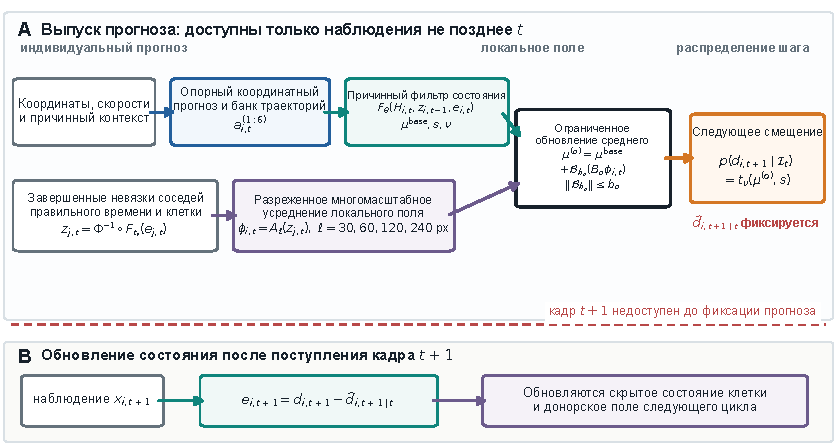
\includegraphics[width=\textwidth]{figures/fig2_architecture.pdf}
\caption{Итоговая архитектура и причинный порядок поступления информации. Координатный модуль строит опорный прогноз и банк специализированных остаточных траекторий; фильтр состояния выдает базовое условное среднее, масштаб и степень свободы распределения Стьюдента. Отдельная разреженная ветвь агрегирует только завершенные невязки соседей правильного времени и идентичности. Регуляризованный линейный оператор добавляет ограниченную поправку к среднему, не изменяя масштаб вероятностного прогноза. Верхняя часть соответствует выпуску и фиксации прогноза до кадра $t+1$; нижняя часть показывает допустимое обновление после поступления этого кадра.}
\label{fig:architecture}
\end{figure}

\section{Результаты}
\subsection{Архитектурный поиск выявил различие между покрытием и наблюдаемостью}
Архитектурный поиск был организован как последовательность диагностических проверок, а не как турнир моделей по одной итоговой метрике. Сначала оценивалось геометрическое покрытие: содержит ли порожденный набор траекторий вариант, близкий к истинному будущему. Затем проверялась прогностическая наблюдаемость, то есть возможность по данным, доступным до следующего кадра, определить, какой вариант реализуется. Наконец, для каждого нового источника данных оценивалось добавочное содержание: превосходит ли реальный признак нулевой, перемешанный по времени и принадлежащий другой клетке контроль. Такое разделение оказалось принципиальным, поскольку хорошее покрытие еще не означает наблюдаемость правильного класса движения.

В исходной постановке шесть будущих шагов строились из одной фиксированной точки. Смеси распределений, условный генератор со скрытыми переменными и диффузионный остаток уменьшали минимальную ошибку среди 32 кандидатов приблизительно на 5-10\%. Однако выигрыш исчезал при переходе от знания лучшего кандидата после опыта к выбору до наблюдения будущего. Под модулем выбора траектории здесь понимается модель, которая получает все кандидаты и доступный контекст, присваивает им веса и формирует одно итоговое смещение до появления целевого кадра. Были проверены линейные оценки, модели множеств, внимание между кандидатами, графовая оценка и последовательное уточнение. Ни один вариант не переносил улучшение минимальной ошибки в устойчивое уменьшение конечной RMSE относительно согласованных случайных контролей. Следовательно, основной недостаток заключался не в отсутствии разнообразных будущих траекторий, а в отсутствии наблюдаемого признака, позволяющего заранее выбрать нужную.

Этот вывод был проверен учителем, которому во время обучения открывался истинный будущий остаток. Учитель уверенно разделял режимы направления, поворота и скорости; при перемешивании будущего структура разрушалась. Ученик, получавший только прошлое и текущий контекст, не воспроизводил эти режимы лучше перемешанного контекста. Линейные и динамические разложения, спектральные представления, тензорная факторизация, разреженные и вариационные автокодировщики, а также отдельные последовательные кодировщики компонент улучшали описание уже известного будущего, но не сокращали разрыв между учителем и учеником. Тем самым была локализована проблема: скрытые режимы существуют как удобное описание результата, но их нельзя восстановить одним лишь увеличением размерности скрытого пространства.

Отдельная проверка оценивала возможность заменить недостающий признак законом взаимодействия. Статические парные функции $c(r)$, эффективные потенциалы и набор условных парных признаков $C(1,2)$, включавший расстояние, относительную скорость, плотность, границу, локальный поток и топологию, обнаруживали грубо неправдоподобные конфигурации, но не определяли знак следующего остаточного вектора. Полный набор ухудшил h6 на 2,99\% в MDCK Bulk и на 1,58\% в MDCK Edge относительно лучшего контроля. Радиальная передача сообщений давала небольшой выигрыш над чистым собственным потоком, однако он не сохранялся при строгом сравнении с перемешанным соседством. Поэтому граф не был принят как свободная модель неизвестной силы. Позднее он получил более узкую роль: переносить уже измеренную невязку завершенного перехода, не пытаясь вывести ее из одной геометрии.

Наконец, проверялась гипотеза о недостающей модальности. Сначала была исправлена процедура сопоставления идентичностей клеток между треками и изображениями; доля корректно сопоставленных временных пар выросла с 2,1 до приблизительно 97,5\%. После этого локальные и многомасштабные окна, псевдомаски и сегментация, DINOv2, временное самообучение, форма, полярность, свободное пространство, контакт и коридор возможной траектории сравнивались с изображением другой клетки, тем же кадром другой клетки и перемешанным временем. Признаки надежно описывали внешний вид, но не давали добавочного прогноза индивидуального остатка. Измеренные тяга и напряжение также не прошли перенос на LaChance, хотя искусственная проверка показала, что используемый передаточный слой способен обнаружить сигнал заданной силы. В общей матрице из 23 проверок мощности, чувствительности и переноса ни один самостоятельный модуль переноса новой модальности не прошел одновременно все заранее заданные критерии включения в условное среднее. Исходные косвенные морфологические и наблюдательные признаки опорного координатного прогноза при этом не удалялись; отрицательный вывод относится к новым самостоятельным визуальным, сегментационным и механическим поправкам среднего.

Отдельный внешний опыт на трех двухканальных последовательностях LifeAct-MDCK уточнил этот вывод \cite{ref34}. CPSAM-маски, причинно связанные между кадрами и дополненные полярностью актина, геометрией контакта и показателями надежности, не улучшили среднее смещение при исключении целой последовательности: h1 RMSE составила 11,082 против 11,068 пикселя у координатного варианта. Однако при замороженном координатном среднем те же признаки уменьшили Student-$t_4$ NLL с 3,649 до 3,614; лучший временной, межклеточный, строковый или нулевой контроль имел NLL 3,644. Безразмерная проверка по текущему диаметру клетки сохранила направление эффекта, 3,682 против 3,657. Следовательно, явное клеточное состояние оказалось полезно для оценки масштаба ошибки, но не для направления следующего остатка. Этот результат является исследовательским из-за трех независимых условий и отсутствия ручных треков и не меняет зафиксированное среднее основной модели.

Таким образом, отрицательные опыты не просто сократили число модулей. Они последовательно исключили три объяснения потолка: недостаточное покрытие пространства будущего, недостаточную емкость представления и отсутствие достаточно сложной статической функции соседства. После этого объект прогнозирования был изменен с ненаблюдаемого будущего режима на уже реализованное отклонение от сильного индивидуального прогноза. Это отклонение становится доступным только после завершения перехода и потому может использоваться без утечки для следующего шага.


\begin{table}[H]
\centering
\caption{Диагностические развилки архитектурного поиска. Каждый вывод основан не только на конечной ошибке, но и на контроле, различающем информацию, доступную до прогнозируемого перехода, геометрическое покрытие и емкость модели. Отрицательный результат проверки не отрицает биологического содержания признака.}
\label{tab:search}
\small
\begin{tabularx}{\textwidth}{@{}L{0.19\textwidth} Y L{0.24\textwidth} L{0.13\textwidth}@{}}
\toprule
Проверяемая гипотеза & Диагностическое наблюдение & Фальсифицирующий контроль & Следствие \\
\midrule
Статическая $c(r)$ & Описывает среднюю плотность, но не сохраняет направление и историю контакта. &
Перемешанное соседство не дает логичного провала. & Исключена \\
Условная $C(1,2)$ & Расстояние, относительная скорость, поток, граница и топология не задали знак остатка. &
Изменение h6: Bulk $-2{,}99\%$, Edge $-1{,}58\%$. & Исключена \\
MDN, CVAE, диффузия & Лучший из 32 кандидатов улучшался примерно на 5--10\%, но выбор кандидата до наблюдения цели не переносил выигрыш в конечную RMSE. &
Модули оценки траекторий не превосходили согласованные случайные контроли устойчиво. & Только покрытие \\
Учитель и разложение сигнала & Будущее разделяло режимы направления, поворота и скорости; ученик, получавший только прошлое, не восстанавливал их. &
Перемешивание будущего разрушало представление учителя, тогда как распределение ученика оставалось слабым. & Не используется для прогноза \\
Видео, маски, механика & После исправления идентичности самостоятельные ветви описывали клетку, но не следующий индивидуальный остаток. &
Ни одна из 23 проверок не прошла одновременно критерии мощности, идентичности и переноса. & Новые ветви не включены \\
LifeAct-состояние & Явные форма, полярность, контакт и надежность не улучшили среднее, но предсказывали масштаб ошибки. &
Student-$t_4$ NLL в межусловной проверке: 3,649 без состояния и 3,614 с реальным состоянием; подмены хуже. & Только оценка неопределенности \\
Завершенная невязка & Остаток согласован у близких клеток, убывает с расстоянием и зависит от правильных времени и идентичности. &
Реальная $<$ устаревшая $<$ другая клетка по h6 RMSE; эффект 6/6 фильмов. & Сохранена \\
\bottomrule
\end{tabularx}
\end{table}

\subsection{Завершенные невязки обнаруживают локально согласованное динамическое поле}
После исключения непрошедших ветвей мы исследовали ошибку сильного последовательного одношагового прогноза. Пусть $d_{i,t}=x_{i,t}-x_{i,t-1}$ обозначает уже состоявшееся смещение клетки $i$, а $\widehat d_{i,t\mid t-1}$ - прогноз этого смещения, сохраненный до появления кадра $t$. Завершенная невязка определяется как

\begin{equation}
e_{i,t}=d_{i,t}-\widehat d_{i,t\mid t-1}.
\end{equation}
Эта величина содержит только информацию о завершенном переходе. Она недоступна для прогноза $t-1\rightarrow t$, но становится допустимым входом при выпуске прогноза $t\rightarrow t+1$. Пространственный анализ на рис. 3A является ретроспективной диагностикой уже завершенных ошибок, а не признаком того же прогнозируемого перехода. Предсказания трех инициализаций сначала усреднялись внутри каждого исключенного фильма; независимыми единицами оставались шесть фильмов. Для каждой клетки ближайшие соседи сравнивались со случайными клетками того же кадра, что исключало общий сдвиг фильма и различие временных условий.

У близких клеток невязки были согласованы сильнее, чем у случайных клеток того же кадра. Для одного ближайшего соседа нормированный избыток скалярного произведения составил $0{,}316\pm0{,}037$; при восьми соседях он сохранился на уровне $0{,}186\pm0{,}020$. Избыток косинусного сходства и покомпонентной корреляции имел ту же монотонно убывающую зависимость от среднего расстояния. Знак избытка был положительным на всех шести фильмах. Наличие трех согласующихся мер важно: эффект нельзя объяснить только общей амплитудой ошибки или только совпадением углов.

Информационная лестница на семи фильмах MDCK Bulk 10--16, не использованных для выбора текущей конфигурации, затем проверила, переходит ли диагностическая корреляция в последовательный прогноз. Эти фильмы участвовали в более раннем широком поиске проекта, поэтому проверка является замороженной относительно текущей архитектуры, но не полностью гипотезно-наивной. Для режима ближайшего шага базовая модель имела h6 RMSE 6,496. Собственная завершенная невязка уменьшила ее до 6,217. Добавление локальных невязок соседей дало 5,773, то есть добавочно уменьшило ошибку на 0,444 пикселя. Средняя поправка всего кадра снизила показатель лишь до 5,682, еще на 0,091 пикселя. Следовательно, основная добавочная информация была локальной, а не следствием общего дрейфа изображения.

В накопительном режиме временные и идентификационные контроли определили границу интерпретации. Актуальная невязка правильной клетки дала h6 RMSE 4,820, невязка той же клетки из более раннего времени - 5,565, базовой вероятностной модели без локального переноса - 6,496, а невязка другой клетки - 7,279. Внутреннее последовательное обновление базового фильтра при этом не отключалось. При подмене сохраняются правдоподобные масштабы и плотность значений, но нарушается соответствие конкретному времени или клеточной идентичности. Такое упорядочение показывает, что модель использует не произвольную остаточную поправку, а текущую локальную реализацию поля.

Мы интерпретируем этот результат осторожно. Невязка может смешивать неописанную биологическую динамику, локальное движение ткани и коррелированную ошибку измерения; она не является прямой оценкой силы. Однако пространственное затухание, превосходство над случайной клеткой того же кадра и отдельный добавочный вклад соседей отвергают объяснение одной постоянной поправкой. Поэтому итоговый граф не выводит физический закон из расстояний. Он выполняет более проверяемую операцию: переносит ограниченную статистику уже завершенного локального возмущения на следующий последовательный прогноз.


\begin{figure}[tb]
\centering
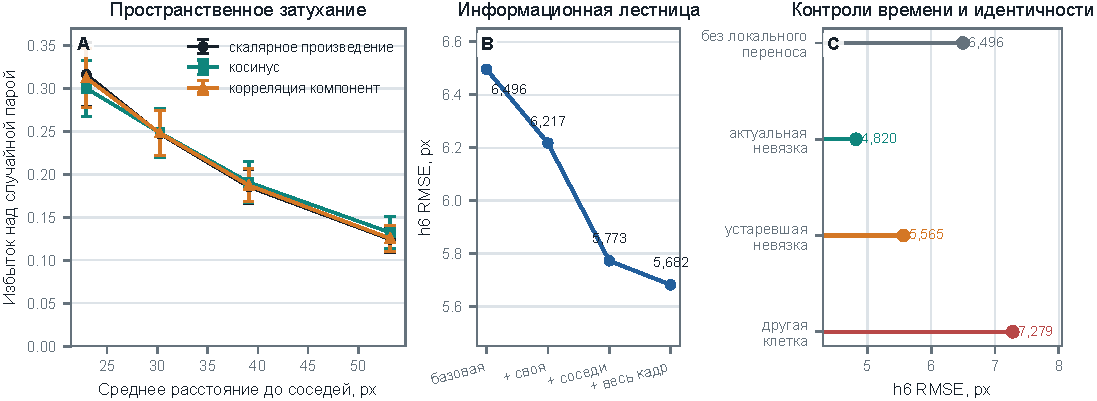
\includegraphics[width=\textwidth]{figures/fig3_innovation_evidence.pdf}
\caption{Диагностика завершенной невязки. \textbf{A}, избыток согласованности относительно случайной клетки того же кадра убывает с расстоянием (среднее $\pm$ стандартное отклонение по фильмам). \textbf{B}, информационная лестница на фильмах MDCK Bulk 10--16, не использованных для выбора текущей конфигурации. \textbf{C}, временные и идентификационные контроли внешнего локального переноса; последовательное обновление базового фильтра остается включенным во всех вариантах.}
\label{fig:innovation}
\end{figure}

\subsection{Невязка задает приближенную кинематическую оценку коллективного возмущения}
На масштабе одного межкадрового шага точное разложение биологического движения на собственную поляризацию, тканевый поток, механику контакта и ошибку центроида по одним трекам не идентифицируется. Поэтому мы используем более узкое операционное разложение

\begin{equation}
d_{i,t+1}
=
\mu^{\mathrm{base}}_{i,t+1}
+c^{(o)}_{i,t+1}
+\varepsilon_{i,t+1},
\qquad
c^{(o)}_{i,t+1}
=
\mathcal B_{b_o}\!\left(B_o\phi_{i,t}\right).
\end{equation}
Здесь $\mu^{\mathrm{base}}$ является прогнозом индивидуального последовательного фильтра, $c^{(o)}$ -- условно предсказуемой пространственно коррелированной компонентой его невязки, а $\varepsilon$ объединяет непредсказанную активную изменчивость, ошибку модели и ошибку сопровождения. Индекс $o$ обозначает рабочую точку ближайшего шага или накопительной последовательности. Это разложение согласуется с представлением коллективной миграции как активной среды с памятью \cite{ref2,ref3,ref4}, но не утверждает, что $c^{(o)}$ является отдельной силой, тканевой скоростью или консервативным полем.

Вход $\phi$ строится не из физических невязок напрямую. Для каждой компоненты завершенная ошибка сначала преобразуется через функцию распредения Стьюдента в нормальную оценку $z=\Phi^{-1}[F_{t_\nu}((d-\mu)/s)]$. Набор признаков объединяет собственную предыдущую оценку $z$, ее доступность, среднее по кадру, локальные средние, покомпонентные стандартные отклонения и эффективное число соседей на четырех масштабах, а также взаимодействия этих величин с двумя компонентами прогнозного масштаба. Только результат $B_o\phi$ после обратной калибровки имеет размерность смещения за кадр.

Поэтому физически корректнее называть $c^{(o)}$ приближенной кинематической оценкой коллективного возмущения или поправкой локального переноса. Пространственное затухание на рис. 3A указывает на характерную длину согласованности; превосходство актуальной невязки над устаревшей указывает на короткую временную память; малый добавочный вклад среднего по кадру отделяет локальную компоненту от общего дрейфа изображения. Определение корреляции и способ оценки ее длины могут заметно менять численное значение масштаба даже для одного поля \cite{ref31}; поэтому ниже отдельно сообщаются непараметрическая длина затухания и экспоненциальная аппроксимация, а междоменная универсальность не предполагается заранее. Распределение Стьюдента описывает оставшиеся тяжелохвостые активные флуктуации и ошибки сопровождения, но не должно интерпретироваться как тепловой шум.

Переход от такого поля смещений к силе потребовал бы одновременных измерений тяги или напряжения и калиброванного соотношения сила-скорость, как в интервенционных механических экспериментах \cite{ref3,ref4,ref24}. Проверенный межэкспериментальный перенос этих величин на LaChance не прошел критерий включения. Следовательно, статья обосновывает кинематическую коллективную составляющую, но намеренно не заявляет восстановление механической силы, давления или энергии.

\subsection{E(2)-эквивариантная модель поля отделяет кинематику от механики}
Чтобы проверить, не скрывает ли локальный перенос более простой полевой закон, мы использовали независимый набор из 22 ограниченных островков MDCK с одновременными полями скорости, тяги к субстрату и напряжения монослоя \cite{ref24}. Низкая и высокая плотность, ингибирование актомиозина CytoD и активация Rho с помощью CN03 образовали отдельные островковые группы. Пусть $v_t$ обозначает поле скорости прогнозируемого перехода, а $u_t=v_t-v_{t-1}$ -- его приращение относительно завершенной скорости. На момент прогноза доступно $u_{t-1}$, поэтому проверялся причинный закон

\begin{equation}
\begin{aligned}
\widehat u_t={}&
a\,u_{t-1}
+\nu_T\nabla^2u_{t-1}
+\nu_L\nabla(\nabla\!\cdot u_{t-1})
+\lambda_v(v_{t-1}\!\cdot\nabla)u_{t-1}\\
{}&
+\lambda_u(u_{t-1}\!\cdot\nabla)u_{t-1}
-g\|u_{t-1}\|^2u_{t-1}
+b\,n_\partial e^{-d_\partial/\ell_\partial}
+c_TT+c_\sigma\nabla\!\cdot\sigma+c_FF .
\end{aligned}
\label{eq:field_law}
\end{equation}

Все коэффициенты являются скалярами, общими для двух компонент вектора; свободный лабораторный вектор и отдельные коэффициенты для $x$ и $y$ не допускаются. Поэтому непрерывная библиотека эквивариантна относительно переносов, поворотов и отражений. Производные вычислялись на исходной полной сетке поля до пространственного прореживания. Внешний цикл исключал целый островок, а параметры регуляризации и разреживания выбирались на другом целом островке.

Обученное скалярное затухание $a\,u_{t-1}$ уменьшило покомпонентную RMSE скорости с 0,118236 до 0,109476 $\mu$m/min, или на 8,110\%. Добавление лапласиана, продольно-поперечного члена, двух адвекций и кубического насыщения снизило RMSE до 0,108466, то есть дало 8,829\% относительно постоянства скорости и добавочные 0,767\% относительно скалярного затухания. Добавочный эффект был положительным в 20/22 островков, точный односторонний знаковый тест $p=6{,}06\cdot10^{-5}$. Исключения сосредоточены в двух островках высокой плотности; средний добавочный эффект в этой группе был отрицательным. Временная подмена, поле другого островка и пространственный сдвиг дали соответственно $-0,015$, 0,034 и 0,673\% относительно постоянства скорости. Следовательно, основная часть 8,829\%-эффекта требует правильной пространственно-временной реализации поля.

\begin{center}
\captionof{table}{Проверка E(2)-эквивариантного полевого закона с исключением целого островка на наборе с измеренной механикой. RMSE выражена в $\mu$m/min. Процент рассчитан относительно прогноза постоянной скорости в том же внешнем цикле.}
\label{tab:field_law}
\small
\begin{tabularx}{\textwidth}{@{}Y r r L{0.31\textwidth}@{}}
\toprule
Вариант & RMSE & Изменение & Интерпретация \\
\midrule
Постоянство скорости & 0{,}118236 & 0{,}000\% & причинная опорная модель \\
Обученное скалярное затухание & 0{,}109476 & $-8{,}110$\% & временная память без производных \\
Адвективный полевой закон & 0{,}108466 & $-8{,}829$\% & полный кинематический пакет \\
Пространственный сдвиг поля & 0{,}117356 & $-0{,}673$\% & нулевой контроль \\
Временная подмена поля & 0{,}118212 & $+0{,}015$\% & нулевой контроль \\
Поле другого островка & 0{,}118047 & $-0{,}034$\% & нулевой контроль \\
Продольно-поперечный закон без механики & 0{,}109004 & $-8{,}444$\% & симметрийно согласованный кинематический контроль \\
Тот же закон с тягой и напряжением & 0{,}109006 & $-8{,}440$\% & добавочная механика отсутствует \\
\bottomrule
\end{tabularx}
\end{center}

\begin{center}
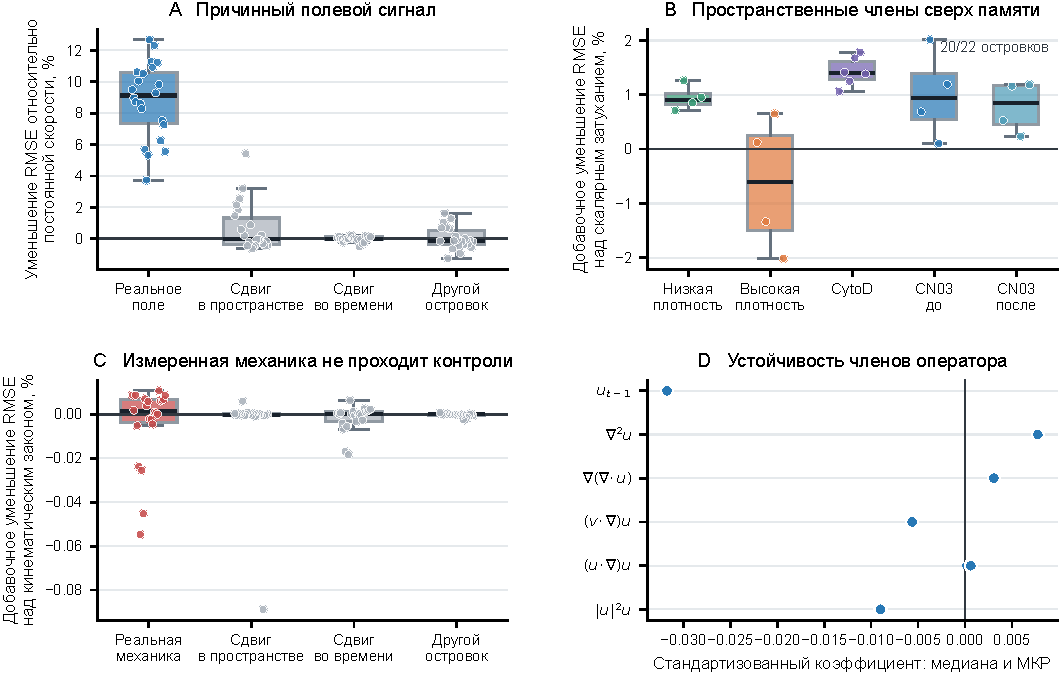
\includegraphics[width=0.84\textwidth]{figures/fig7_equivariant_field_law.pdf}
\captionof{figure}{Проверка E(2)-эквивариантного полевого закона на 22 островках MDCK. \textbf{A}, уменьшение RMSE адвективным законом и его пространственно-временные и межостровковые контроли. \textbf{B}, добавочный эффект пространственных членов над обученным скалярным затуханием по экспериментальным группам. \textbf{C}, измеренная механика не улучшает симметрийно согласованный кинематический закон и не превосходит подмены. \textbf{D}, медианы и межквартильные размахи стандартизованных коэффициентов в 22 внешних циклах; нулевое значение означает исключение члена внутренней разреживающей процедурой. Знаки устойчивы для $u_{t-1}$, лапласиана, продольно-поперечного члена, адвекции скоростью и кубического насыщения, но сами коэффициенты не трактуются как механические параметры.}
\label{fig:field_law}
\end{center}

Измеренная механика не прошла более строгую проверку. Тяга, дивергенция напряжения и их баланс не улучшили согласованный продольно-поперечный закон; временная, пространственная и межостровковая подмены дали тот же результат. В обратной задаче добавление завершенной невязки к скорости изменило RMSE восстановления тяги и дивергенции напряжения в среднем на $-0,010$\%, а $R^2$ оставался отрицательным. При переносе между плотностями и до/после CytoD или CN03 реальная механика уступила кинематическому закону на 0,103\% и лучшему механическому контролю на 0,110\%. Ошибка продольно-поперечного динамического спектра уменьшилась лишь на 0,052\%. На синтетических полях та же реализация восстановила известные коэффициенты с медианной ошибкой 0,38\% и покрытием 6/6 истинных коэффициентов 95\%-интервалами; алгебраический произвольный поворот и сеточный поворот на $180^\circ$ дали относительную ошибку ниже $10^{-10}$. Поэтому отрицательный механический вывод не объясняется неспособностью регрессии обнаружить заданный закон.

Таким образом, внешний полевой опыт усиливает кинематическую часть интерпретации: локальное остаточное поле подчиняется воспроизводимой симметрийно согласованной динамике, которая не сводится к одной памяти. Одновременно он закрывает более сильную формулировку: эти данные не позволяют отождествить найденный оператор с тягой или напряжением. Такое разделение соответствует требованию обучения уравнений активной материи проверять не только точечную ошибку, но также симметрии, спектры и перенос между режимами \cite{ref32}.

\FloatBarrier
\subsection{Полевой закон допускает эффективный диссипативный функционал}
Часть найденного оператора допускает вариационную запись. Перепишем причинную карту для изменения поля приращения скорости как

\begin{equation}
u_t-u_{t-1}
=
-\frac{\delta\mathcal F_{\mathrm{eff}}}{\delta u}
+\mathcal A[u,v]
+\varepsilon_t ,
\end{equation}

где неравновесный перенос $\mathcal A$ содержит адвективные члены, а

\begin{equation}
\mathcal F_{\mathrm{eff}}[u]
=
\int_\Omega
\left[
\frac{r}{2}\|u\|^2
+\frac{g}{4}\|u\|^4
+\frac{K_T}{2}\|\nabla u\|_F^2
+\frac{K_L}{2}(\nabla\!\cdot u)^2
\right]\,dx .
\label{eq:effective_functional}
\end{equation}

Отрицательная вариационная производная этого функционала дает $-ru-g\|u\|^2u+K_T\nabla^2u+K_L\nabla(\nabla\!\cdot u)$. Для прямой карты $u_t=a u_{t-1}+\ldots$ выполняется $r=1-a$. Мы повторили внешне-островковую оценку с ограничениями $r>0$, $g\geq0$, $K_T\geq0$ и $K_L\geq0$. Ограничения оказались неактивными: свободная и ограниченная оценки совпали, а функционал был ограничен снизу во всех 22 внешних циклах.

Градиентный сектор без адвекции достиг одношаговой RMSE 0,108610 $\mu$m/min и уменьшил ошибку постоянной скорости на 8,704\%, сохранив 98,6\% выигрыша полного адвективного закона. Полный закон имел RMSE 0,108466 и был лучше в 14 из 22 островков, однако его преимущество 0,133\% не было подтверждено знаковым тестом ($p=0{,}143$). Направление градиентного обновления имело средний косинус 0,701 с наблюдаемым изменением и $-0,001$ после временной перестановки. Эта диагностика первого порядка еще не доказывает уменьшение функционала за конечный шаг.

Поэтому мы дополнительно вычислили точную разность $\mathcal F_{\mathrm{eff}}[u_{\mathrm{new}}]-\mathcal F_{\mathrm{eff}}[u_{\mathrm{old}}]$ на полной сетке каждого тестового островка. Конечное обновление потенциальной модели уменьшало функционал во всех 398 кадрах: средняя разность равна $-0{,}0405$. Для наблюдаемого перехода средняя разность была $-0{,}00794$, но уменьшение происходило только в 51,3\% кадров против 49,2\% при временной перестановке; на уровне островков наблюдаемый переход превосходил перестановку лишь в 7/22 случаев. Следовательно, конечная диссипативность подтверждена как свойство обученной карты, но не как закон наблюдаемой ткани.

Последовательное развертывание проверяло, сохраняется ли польза закона за пределами одного локального шага. При замороженной на момент выпуска границе потенциальная модель уменьшила RMSE постоянства скорости с 0,127648 до 0,117899 на h1 и с 0,167648 до 0,158442 на h6, то есть на 8,29 и 6,30\% соответственно; эффект был положительным в 22/22 исключенных островках. Адвективный вариант дал практически те же значения 0,117831 и 0,158348. Значит, потенциальный сектор является не только локальной аппроксимацией производной, но и устойчивым конечным оператором на проверенной шестишаговой шкале.

Эта конструкция допускает энергетический язык только в ограниченном математическом смысле. $\mathcal F_{\mathrm{eff}}$ является функционалом поля кинематического приращения, определенным с точностью до неизвестной подвижности и масштаба времени. Адвекция задает циркулирующий неравновесный поток и в общем случае не является градиентом скалярного потенциала. Поскольку наблюдаемое уменьшение не превзошло временную перестановку, а тяга и напряжение не прошли критерий механического переноса, $\mathcal F_{\mathrm{eff}}$ нельзя называть энергией клетки, деформации, контакта или ткани и нельзя выражать в физических единицах энергии. Корректная интерпретация -- ограниченный снизу эффективный функционал потенциальной части кинематической модели.

\subsection{E(2)-эквивариантный закон воспроизводит полезную часть итогового графа}
Внешняя полевая проверка и итоговая модель используют разные представления: непрерывные производные поля и статистики соседских невязок соответственно. Чтобы проверить, не является ли их сходство лишь словесной аналогией, мы заменили свободную плотную поправку LaChance ограниченной графовой библиотекой. В нее вошли собственная и средняя по кадру завершенные невязки, продольные и поперечные соседские компоненты на трех масштабах, кубическое насыщение и, только в активном варианте, две адвективные компоненты. Каждая векторная функция имела один скалярный коэффициент, общий для $x$ и $y$; свободный лабораторный вектор и покомпонентные коэффициенты были запрещены. Потенциальный вариант дополнительно фиксировал знаки релаксации, пространственного сглаживания и насыщения. Все доноры относились к завершенному переходу $t-1$, а вращение и отражение библиотеки воспроизводились с максимальной ошибкой ниже $10^{-9}$.

На шести внешних циклах потенциальный закон объяснил 81,1\% дисперсии плотной поправки режима ближайшего шага и 95,1\% дисперсии поправки накопительного режима. Для h6 он достиг RMSE 6,754 при строгой h1-точке и 5,581 при накопительной точке против 6,785 и 5,501 у свободного плотного оператора; тем самым сохранено соответственно 103,0 и 96,5\% его выигрыша над моделью без локального переноса. В обоих режимах h6 улучшился в 6/6 фильмах. На h1 потенциальный закон дал 3,470 пикселя и не установил преимущества: улучшение наблюдалось только в 3/6 фильмах.

\begin{table}[H]
\centering
\caption{Замороженная проверка E(2)-эквивариантного потенциального графового закона на фильмах MDCK Bulk 10--16. Параметры и ограничение нормы выбраны только по перекрестной проверке внутри фильмов 1--6. Процент -- среднее фильмовых улучшений относительно базовой вероятностной модели без локального переноса.}
\label{tab:equivariant_bridge}
\small
\setlength{\tabcolsep}{4.5pt}
\begin{tabularx}{\textwidth}{@{}Y r r r r r@{}}
\toprule
Рабочая точка & h1 RMSE & h6 RMSE & $R^2$ h6 & Выигрыш h6 & Положит. \\
\midrule
Ближайший шаг & 3{,}416 & 5{,}759 & 0{,}932 & 11{,}36\% & 7/7 \\
Накопительная последовательность & 3{,}716 & 4{,}842 & 0{,}952 & 25{,}46\% & 7/7 \\
\bottomrule
\end{tabularx}
\end{table}

В замороженной проверке на фильмах 10--16 потенциальный закон улучшил h6 в 7/7 фильмах для обеих рабочих точек (табл.~\ref{tab:equivariant_bridge}). Для накопительной точки актуальная невязка правильной клетки превосходила неправильную клетку в среднем на 2,529 пикселя и устаревшее время на 0,686 пикселя, также в 7/7 фильмах. Точное двустороннее значение для h6 равно 0,015625, а односторонняя поправка Холма по четырем горизонтам -- 0,03125. Ограниченная библиотека почти воспроизводит лучшую свободную поправку, но не заменяет ее в основной таблице: h6 RMSE 4,842 остается немного выше итогового значения 4,820. Ее роль -- проверяемая связь между прогностическим графом и симметрийно согласованной полевой интерпретацией.

\subsection{Масштаб поля направляет локализацию оператора}
Для количественного выбора опоры мы рассчитали лаговую межклеточную корреляцию причинно доступных, аффинно детрендированных нормальных оценок невязки $\widetilde z$. Сначала для каждого кадра вычислялось
\begin{equation}
K_z(r,\tau)=
\frac{
\left\langle \widetilde z_{i,t+1}\cdot
\widetilde z_{j,t+1-\tau}\right\rangle_{\|x_i-x_j\|\in r}
}{
\sqrt{
\left\langle\|\widetilde z_{i,t+1}\|^2\right\rangle_r
\left\langle\|\widetilde z_{j,t+1-\tau}\|^2\right\rangle_r
}
}
\end{equation}
в неперекрывающихся интервалах расстояния, после чего кадровые оценки усреднялись. Корреляция ближайшего интервала при задержке на один кадр составила 0,0516 с 95\% интервалом [0,0458; 0,0580] на шести разработческих фильмах и 0,0199 [0,0138; 0,0266] на отдельной группе из семи фильмов MDCK Bulk 10--16. Знак был положительным соответственно на 6/6 и 7/7 фильмах; пространственная, временная и межфильмовая перестановки уменьшали эффект во всех этих фильмах.

Длина поля оказалась зависимой от способа нормировки. Непараметрическое пересечение уровня $e^{-1}$ имело медиану 3,70 расстояния до ближайшего соседа в разработческой группе и 1,39 во второй группе фильмов MDCK Bulk 10--16. Экспоненциальная аппроксимация в пикселях дала близкие средние 62,4 и 60,2 px, однако во второй группе устойчивая экспоненциальная оценка была получена только для трех из семи фильмов. В HUVEC и MDA-MB-231 обнаруживалась малая положительная средняя корреляция, но межфильмовый контроль был слабее, а в MDCK Edge изотропное среднее не отличалось от нуля. Эти результаты подтверждают локализованную лаговую согласованность в MDCK Bulk, но не доказывают строго конечную опору поля и не подтверждают универсальную безразмерную корреляционную длину для разных клеточных систем.

\begin{table}[H]
\centering
\caption{Междоменная диагностика поля завершенной невязки. $K_1$ обозначает векторную корреляцию аффинно детрендированных нормальных оценок в ближайшем пространственном интервале; $r_e$ -- медианное непараметрическое пересечение уровня $e^{-1}$ в пикселях. Число в скобках показывает долю фильмов с конечной оценкой $r_e$. Направленная структура оценивается отдельно от изотропного среднего.}
\label{tab:field_domains}
\scriptsize
\setlength{\tabcolsep}{3.5pt}
\begin{tabularx}{\textwidth}{@{}L{0.19\textwidth} r L{0.24\textwidth} r r Y@{}}
\toprule
Домен & Фильмы & $K_1$, 95\% интервал & Положит. & $r_e$, px & Направленная структура \\
\midrule
MDCK Bulk, разработка & 6 & 0{,}0516 [0{,}0458; 0{,}0580] & 6/6 & 82{,}5 (6/6) & первая гармоника не воспроизведена во второй группе \\
MDCK Bulk 10--16 & 7 & 0{,}0199 [0{,}0138; 0{,}0266] & 7/7 & 106{,}8 (7/7) & не прошла полный набор контролей \\
MDCK Edge & 15 & 0{,}0017 [$-0{,}0015$; 0{,}0051] & 8/15 & 83{,}8 (14/15) & первая гармоника прошла четыре контроля \\
HUVEC & 18 & 0{,}0045 [0{,}0020; 0{,}0068] & 15/18 & 66{,}1 (10/18) & не подтверждена \\
MDA-MB-231 & 17 & 0{,}0037 [0{,}0025; 0{,}0049] & 15/17 & 91{,}2 (12/17) & не подтверждена \\
\bottomrule
\end{tabularx}
\end{table}

Диагностическая кривая одного запуска показывала насыщение основной части выигрыша уже около $R=\xi$. Эта оценка не совпала с минимальным надежным радиусом в более строгой трехинициализационной проверке: варианты $2\xi$ и $3\xi$ не сохранили обе рабочие точки в пределах допуска 0,2\%. Поэтому масштаб поля использовался как единица локализации, а не как доказанный универсальный оптимум. Консервативный радиус $R=4\xi$, где $\xi$ оценивалась только по обучающим фильмам внешнего цикла, прошел критерий одновременно для h1 и h6 в двух зафиксированных режимах. В режиме ближайшего шага h1 RMSE изменилась с 3,4744 до 3,4753, а h6 -- с 6,7846 до 6,7721 px. В накопительном режиме соответствующие значения изменились с 3,8080 до 3,8132 и с 5,5007 до 5,4934 px. Разреженная версия использовала в среднем 38,3\% допустимых межклеточных ребер и сохраняла ожидаемый порядок контролей на всех шести внешних фильмах.

Радиусный поиск дал измеренную зависимость времени, близкую к линейной: для итоговой опоры $R=4\xi$ показатель степенной аппроксимации равен 1,079 против 2,043 для плотного попарного расчета. При 10\,000 клеток измеренное ускорение составило 30,68 раза. Для 50\,000 клеток граф содержал 3,98 млн ребер, а построение и применение оператора заняли 1,14 с; плотное время для этого размера не экстраполировалось. Это не означает, что усеченный пакет является поточечной копией каждого плотного признака. Для широкого исторического масштаба 240 px при $R=4\xi$ сохранялось в среднем 62,4\% массы ядра, тогда как после повторной оценки линейного оператора итоговый прогноз оставался внутри заданного допуска неухудшения. Следовательно, разреженная версия является обученной локальной параметризацией того же интерфейса, а не простой численной отсечкой готовой плотной поправки.

Внешняя проверка разреженной параметризации выполнялась только после точного воспроизведения плотных результатов исходной сетки гиперпараметров. Для каждого внешнего цикла радиус равнялся четырем медианным непараметрическим длинам $e^{-1}$, оцененным на его обучающих фильмах в пикселях; это доменно адаптивная процедура, а не перенос одной Bulk-константы. Изотропный оператор прошел односторонний допуск h1/h6 и временной и идентификационный контроли в HUVEC, MDA-MB-231 и MDCK Edge. В накопительном режиме h6 RMSE изменилась соответственно с 1,4399 до 1,4258, с 31,3374 до 31,2907 и с 4,7572 до 4,7184 px при использовании 13,4, 9,3 и 3,4\% плотных ребер. На h1 ближайшего шага наибольшее ухудшение составило 0,129\% в Edge. Направленное ядро Edge, несмотря на подтвержденную первую гармонику поля, не превзошло изотропное одновременно в двух рабочих точках; поэтому в итоговую архитектуру оно не включено.

\begin{figure}[tb]
\centering
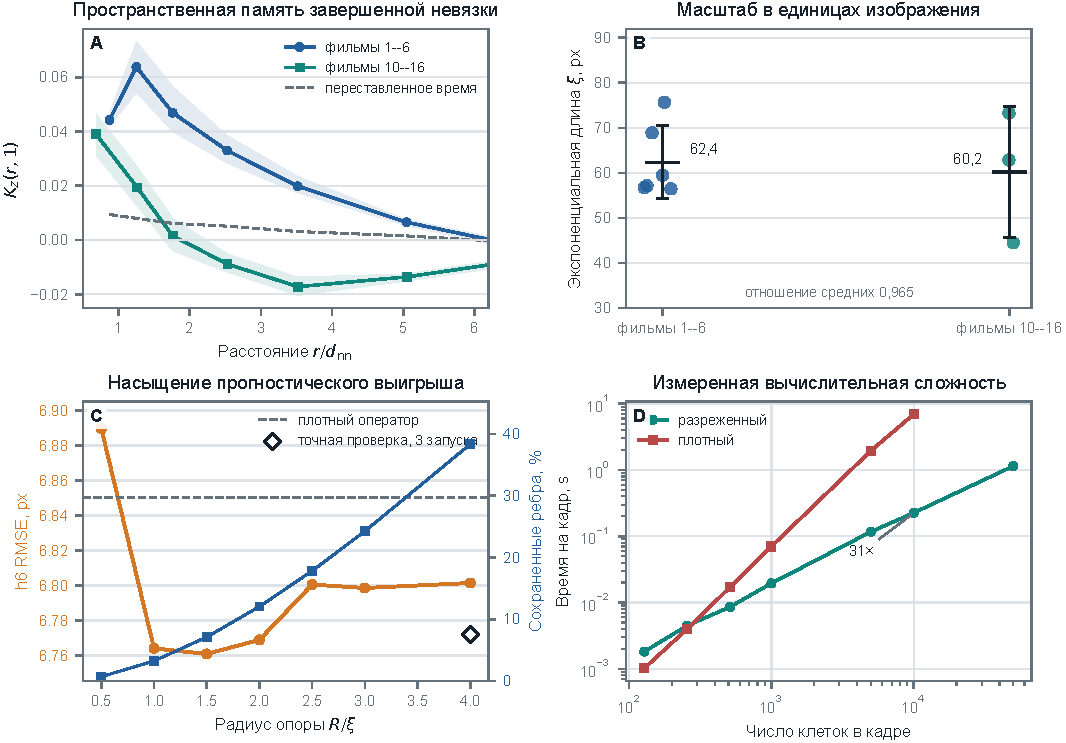
\includegraphics[width=\textwidth]{figures/fig6_field_sparse_operator.pdf}
\caption{Масштаб завершенной невязки и разреженный оператор. \textbf{A}, лаговая корреляция причинно доступных невязок с задержкой в один кадр убывает с расстоянием в разработческих фильмах и в отдельной группе MDCK Bulk 10--16; пунктир показывает временную перестановку. \textbf{B}, диагностические экспоненциальные длины в пикселях; во второй группе конечными были только три аппроксимации, поэтому эта панель не доказывает универсальность масштаба. \textbf{C}, диагностическая кривая h6 для одной инициализации и доля ребер при изменении $R/\xi$; ромб отмечает выбранную затем для точной трехинициализационной проверки опору $R=4\xi$. \textbf{D}, непосредственно измеренное время плотного и радиусного операторов.}
\label{fig:field_sparse}
\end{figure}

На синтетических полях известная длина восстанавливалась с медианной относительной ошибкой 2,49\%, отношение осей анизотропии -- с ошибкой 10,97\%, временная корреляция -- с ошибкой 1,64\%; ложных обнаружений анизотропии в изотропном контроле не было. Вместе с тем покрытие интервалов для пространственной длины и особенно отношения осей не достигло заданного уровня. Поэтому синтетика подтверждает корректность точечных оценок и нулевых контролей, но не дает основания трактовать их интервалы как полностью калиброванные физические доверительные области.

\subsection{Последовательный перенос уменьшает накопительную ошибку}
Основное сравнение использовало внешнее поочередное исключение одного из шести фильмов MDCK Bulk. В каждом цикле один фильм был тестовым, следующий - проверочным, остальные четыре - обучающими. Все методы получали одинаковые упорядоченные примеры и выпускали прогноз до следующего наблюдения. Нейронные модели обучались с тремя инициализациями; статистической единицей оставался фильм.

Сильный априорный прогноз без локального переноса достиг h1 RMSE 3,483, но его накопительная h6 RMSE выросла до 7,812. Режим ближайшего шага предложенного оператора дал h1 RMSE 3,474 и $R^2=0{,}508$. Среднее фильмовых относительных изменений на h1 равно только 0,081\%; отношение двух макро-RMSE соответствует уменьшению на 0,248\%. Эффект наблюдался в четырех из шести фильмов и не был статистически подтвержден: точное двустороннее и скорректированное по Холму значения для гипотезы H1 равны $p=0{,}84375$. Поэтому коллективный модуль не заявляется как существенное улучшение уже сильного ближайшего шага.

Режим последовательности использовал другую точку Парето ограниченного оператора. Ее h1 RMSE 3,808 хуже априорного прогноза на 9,53\%, но h6 RMSE равна 5,501 при $R^2=0{,}938$. Среднее из шести относительных уменьшений ошибки по фильмам составило 29,8\%; эта величина не является отношением двух объединенных RMSE. Улучшение наблюдалось во всех шести фильмах, а средняя парная разность RMSE была 2,311 пикселя с 95\% бутстреп-интервалом [2,206; 2,414]. Для заранее зафиксированной гипотезы H2 точное двустороннее значение равно 0,03125, а поправка Холма по единому семейству H1--H2 дает 0,0625. Таким образом, сильный направленный эффект h6 не пересекает семейный порог 0,05 на шести независимых фильмах. Все остальные горизонты и односторонние проверки считаются вторичными. Накопительная точка была заморожена до расчета результатов отдельной семифильмовой группы; поскольку фильмы 10--16 ранее участвовали в широком разведочном поиске проекта, этот опыт трактуется как проверка замороженной текущей конфигурации, а не как полностью независимое перспективное подтверждение. По сравнению с постоянной скоростью h6 RMSE уменьшилась на 17,4\%; по сравнению с GRU, HGBDT и KalmanNet - на 34,4, 34,5 и 37,5\% соответственно.

Две рабочие точки не следует усреднять в одну цифру. Режим ближайшего шага сохраняет качество h1 и уменьшает h6 до 6,785. Накопительный режим сознательно допускает более крупную одношаговую поправку, чтобы компенсировать систематическое накопление остатка. Они используют одну архитектуру и различаются только ограничением амплитуды, выбранным по проверочному фильму. Высокий $R^2$ на h6 частично связан с большей дисперсией накопленного целевого смещения и не означает, что отдельный следующий шаг стал почти полностью наблюдаемым; поэтому RMSE каждого горизонта остается основной мерой качества.

В таблицах IMM обозначает взаимодействующую смесь кинематических моделей, GRU -- рекуррентную сеть с управляемыми вентилями, а HGBDT -- гистограммный градиентный бустинг по решающим деревьям. Названия KalmanNet и WoLF-IMQ сохранены как названия опубликованных методов.


\begin{table}[tb]
\centering
\caption{Сравнение в едином последовательном протоколе MDCK Bulk без использования будущих наблюдений. RMSE является покомпонентной и выражена в пикселях; h2, h4 и h6 получены суммой прогнозов, каждый из которых выпущен до следующего наблюдения. Для стохастических базовых моделей показано среднее метрик трех инициализаций; для базовой вероятностной и предлагаемых строк сначала усреднены три заранее заданных прогноза, затем вычислены метрики. Поэтому таблица едина по данным и времени, но различие правил ансамблирования учитывается при интерпретации малых различий h1.}
\label{tab:benchmark}
\small
\setlength{\tabcolsep}{4.5pt}
\begin{tabularx}{\textwidth}{@{}Y r r r r r r@{}}
\toprule
Метод & {h1 RMSE} & {h2 RMSE} & {h4 RMSE} & {h6 RMSE} & {$R^2$ h1} & {$R^2$ h6} \\
\midrule
Постоянная скорость & 4{,}292 & 4{,}849 & 5{,}947 & 6{,}657 & 0{,}250 & 0{,}909 \\
IMM: скорость/ускорение & 3{,}945 & 5{,}508 & 7{,}461 & 8{,}825 & 0{,}366 & 0{,}840 \\
GRU по треку & 3{,}628 & 4{,}994 & 6{,}962 & 8{,}412 & 0{,}464 & 0{,}855 \\
HGBDT & 3{,}492 & 4{,}841 & 6{,}860 & 8{,}404 & 0{,}503 & 0{,}855 \\
KalmanNet & 3{,}926 & 5{,}422 & 7{,}473 & 8{,}794 & 0{,}372 & 0{,}840 \\
Базовая вероятностная модель & 3{,}483 & 4{,}692 & 6{,}480 & 7{,}812 & 0{,}506 & 0{,}875 \\
\textbf{Предлагаемая, ближайший шаг} & \textbf{3{,}474} & 4{,}386 & 5{,}733 & 6{,}785 & 0{,}508 & 0{,}905 \\
\textbf{Предлагаемая, накопительный режим} & 3{,}808 & 4{,}181 & 4{,}925 & \textbf{5{,}501} & 0{,}408 & \textbf{0{,}938} \\
\bottomrule
\end{tabularx}
\end{table}

\begin{figure}[tb]
\centering
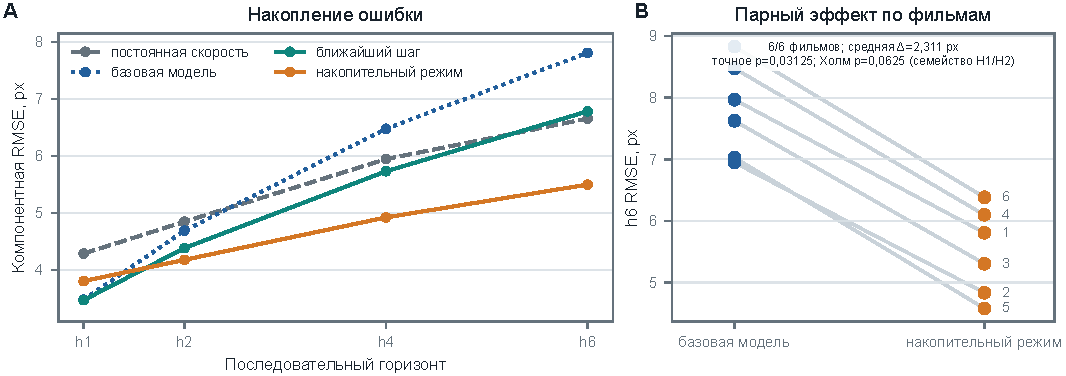
\includegraphics[width=\textwidth]{figures/fig4_primary_results.pdf}
\caption{Основное сравнение MDCK Bulk. \textbf{A}, накопление покомпонентной RMSE в четырех последовательных горизонтах. \textbf{B}, парное изменение h6 RMSE на каждом из шести внешних фильмов относительно той же базовой вероятностной модели без локального переноса.}
\label{fig:primary}
\end{figure}

\subsection{Ближайший шаг является низкосигнальной, но не шумовой задачей}
Низкое значение $R^2$ на h1 нельзя отождествлять с наибольшей абсолютной погрешностью. Для одной и той же рабочей точки ближайшего шага покомпонентная RMSE равна 3,474 px на h1 и 6,785 px на h6, тогда как $R^2$ возрастает с 0,508 до 0,905. Чтобы отделить масштаб цели от ошибки модели, внутри каждого внешнего фильма мы вычислили тождественно следующую из определения $R^2$ величину

\begin{equation}
s_h
=
\frac{\operatorname{RMSE}_h}{\sqrt{1-R_h^2}},
\end{equation}

которая равна стандартному отклонению соответствующей покомпонентной цели при совпадающих выборке и определении метрик. Среднее по шести фильмам $s_h$ составило 4,944 px на h1 и 21,963 px на h6. Таким образом, характерный разброс цели вырос в 4,44 раза, а абсолютная ошибка той же модели -- только в 1,95 раза. Поэтому высокая h6-доля объясненной дисперсии отражает не только качество модели, но и существенно больший знаменатель; значения $R^2$ разных горизонтов не являются прямой шкалой сравнительной трудности.

Эта геометрия метрики согласуется с влиянием локализации центроида. Если наблюдаемая координата имеет вид $\widetilde x_t=x_t+\eta_t$, то измеренное смещение на горизонте $h$ содержит

\begin{equation}
\widetilde D_{t,h}
=
x_{t+h}-x_t+\eta_{t+h}-\eta_t .
\end{equation}

При независимой ошибке локализации ее покомпонентная дисперсия в разности равна $2\sigma_\eta^2$ и не растет пропорционально биологическому смещению. Поэтому на одном кадре тот же порядок ошибки занимает большую долю цели. Во внешнем парном сравнении C2C12 медианное расхождение ручного и автоматического одношагового смещения составило 0,739 px, а 90-й процентиль -- 1,880 px. Эта величина подтверждает чувствительность h1 к сопровождению, но не оценивает неприводимый шум LaChance: значительная часть ручных центроидов C2C12 была интерполирована. Отдельная шестифильмовая проверка LaChance сопоставляла треки с причинно доступной Cellpose-оценкой надежности локализации, однако реальный пакет ухудшил отрицательное логарифмическое правдоподобие на 1,15\% относительно лучшего жесткого контроля и был положителен только в 2/6 фильмах. Независимое повторное сопровождение LaChance не выполнялось. Следовательно, специфический для LaChance нижний предел h1-ошибки не установлен.

Следовательно, h1 не является прогнозом ``из чистого шума'': итоговая модель объясняет около половины его дисперсии и уменьшает абсолютную ошибку относительно постоянной скорости. Нормированная RMSE строгого режима равна 0,702 на h1 против 0,309 на h6; это различие отражает одновременно рост горизонта и масштаба цели. Вместе с тем h1 остается обязательной строгой проверкой причинности. Локальный перенос не дал на нем подтвержденного добавочного преимущества над сильным индивидуальным прогнозом, и этот отрицательный результат не устраняется приведенным анализом отношения сигнал/шум.

Чтобы проверить, не являются ли две выбранные рабочие точки произвольными, до расчета внешних фильмов была задана сетка из 11 функций потерь: вес постепенно переносился от h1 к h6, а допустимое ухудшение h1 на проверочном фильме увеличивалось от 0,5 до 10\%. Коэффициент регуляризации и амплитудное ограничение выбирались только на внутреннем проверочном фильме; внешний фильм использовался один раз. Все 11 точек оказались недоминируемыми по паре h1/h6 и образовали гладкий фронт без скрытого скачка качества (рис. \ref{fig:h1_pareto}). Промежуточные точки являются описательными; подтверждающее семейство включает только крайние заранее зафиксированные гипотезы H1 и H2.

На h1 правильный локальный пакет не отличался от отсутствия переноса, но превосходил невязки другой клетки и устаревшие невязки в 6/6 фильмах; средние парные разности RMSE составили соответственно 0,050 и 0,091 px, точные двусторонние значения $p=0{,}03125$. Это согласуется с наличием слабого причинного локального сигнала, которого недостаточно для заметного улучшения сильного индивидуального h1-прогноза. Для накопительной точки h6 нормированная RMSE равна 0,250, а средняя фильмовая мера навыка относительно постоянной скорости -- 0,315.

\begin{figure}[tb]
\centering
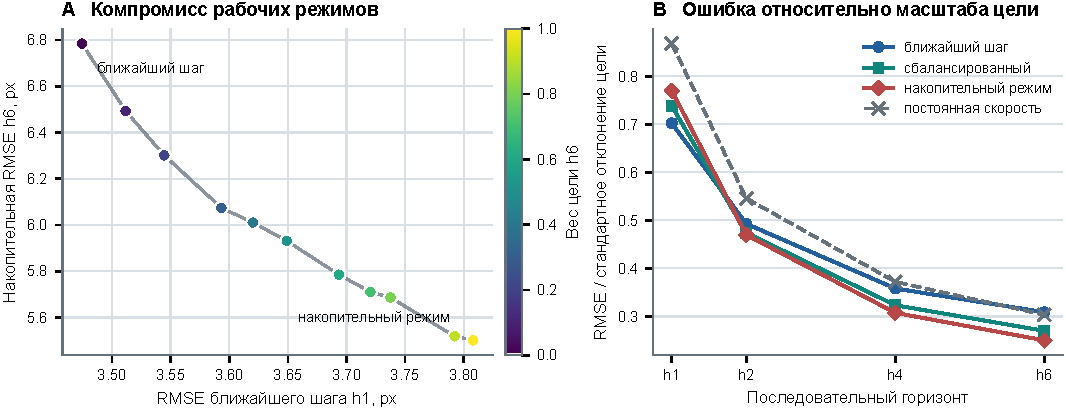
\includegraphics[width=\textwidth]{figures/fig8_h1_pareto_evidence.pdf}
\caption{Строгая проверка ближайшего шага и компромисса горизонтов. \textbf{A}, 11 заранее заданных функций потерь образуют недоминируемый фронт h1--h6; цвет показывает долю перехода от цели ближайшего шага к накопительной цели. \textbf{B}, RMSE, нормированная на восстановленный внутри каждого фильма стандартный разброс цели. Высокое $R^2$ на h6 нельзя непосредственно сравнивать с h1 без учета различного масштаба цели.}
\label{fig:h1_pareto}
\end{figure}

\subsection{Эффект зависит от нового наблюдения и воспроизводится в нескольких доменах}
На семи фильмах MDCK Bulk 10--16 режим последовательности достиг h6 RMSE 4,820 и $R^2=0{,}952$, уменьшив ошибку относительно базовой вероятностной модели без локального переноса на 25,82\%. Средняя парная разность составила 1,676 пикселя с 95\% бутстреп-интервалом [1,620; 1,721]; эффект был положительным в семи из семи фильмов, точное двустороннее непоправленное $p=0{,}015625$. Во вторичном направленном анализе односторонняя поправка Холма по горизонтам h1, h2, h4 и h6 равна 0,03125; эта проверка не смешивается с основным семейством H1--H2 на фильмах 1--6. Конфигурация модели была зафиксирована до расчета этих результатов; фильмы 10--16 ранее использовались только в широком разведочном поиске проекта и не участвовали в выборе текущей конфигурации. Поэтому результат сообщается отдельно от разработческих шести фильмов как проверка замороженной конфигурации, но не называется полностью независимым перспективным опытом. В MDCK Edge нулевой перенос транспортного ядра поверх заранее обученного для Edge базового прогноза дал h6 RMSE $5{,}261\pm0{,}080$, $R^2=0{,}952$ и выигрыш 14,71\% в трех из трех инициализаций; это не является переносом всей модели без дообучения, а неопределенность обозначает стандартное отклонение между инициализациями. Для HUVEC и MDA-MB-231 проверялся другой вид обобщения: одна и та же архитектура заново обучалась внутри каждого внешнего цикла полного вложенного исключения фильма. В HUVEC h6 RMSE составила 1,440 [1,379; 1,515], $R^2=0{,}973$, а выигрыш 11,02\% наблюдался в 18 из 18 циклов. Для MDA-MB-231 ошибка уменьшалась в 17 из 17 циклов на 6,33\%, но абсолютный $R^2=0{,}024$ показывает, что воспроизводимость архитектурного эффекта не равна переносу весов и не устраняет низкую абсолютную предсказуемость этого домена.

Для завершающего сравнения обучаемые базовые методы были заново приведены к тому же временному и выборочному контракту: обучение выполнялось на фильмах 1--4, представление, гиперпараметры и момент остановки выбирались только на фильме 5, после чего три прогноза разных инициализаций усреднялись до расчета метрик на фильмах 10--16. На h1 GRU по треку достигла RMSE 3,362 и $R^2=0{,}507$, HGBDT по трекам -- 3,377 и 0,503, а режим ближайшего шага предложенной модели -- 3,411 и 0,493. Следовательно, преимущество на одном следующем шаге не заявляется. На h6 порядок изменился: HGBDT, GRU и KalmanNet дали RMSE 7,076, 7,689 и 7,789, режим ближайшего шага предложенной модели -- 5,682, а накопительный режим -- 4,820. Для накопительного режима средние парные разности относительно трех обучаемых сравнений составили соответственно 2,256 [2,203; 2,315], 2,869 [2,781; 2,955] и 2,969 [2,850; 3,076] пикселя. Во всех трех случаях эффект имел одно направление в 7/7 фильмах, точное двустороннее $p=0{,}015625$. Эти сравнения не использовались для повторного выбора конфигурации предложенной модели.

\begin{table}[H]
\centering
\caption{Завершающее сравнение обучаемых методов на фильмах MDCK Bulk 10--16. Все модели обучены на фильмах 1--4, а представление, гиперпараметры и момент остановки выбраны только на фильме 5. Для каждого метода три прогноза усреднены до вычисления метрик. HGBDT использует только доступные во всех фильмах координаты, историю скоростей и локальный поток по трекам; недоступные признаки изображений не замещались нулями.}
\label{tab:confirmation_learned}
\small
\setlength{\tabcolsep}{4.2pt}
\begin{tabularx}{\textwidth}{@{}Y r r r r r r@{}}
\toprule
Метод & {h1 RMSE} & {h2 RMSE} & {h4 RMSE} & {h6 RMSE} & {$R^2$ h1} & {$R^2$ h6} \\
\midrule
GRU по треку & \textbf{3{,}362} & 4{,}665 & 6{,}391 & 7{,}689 & \textbf{0{,}507} & 0{,}879 \\
HGBDT по трекам & 3{,}377 & 4{,}415 & 5{,}925 & 7{,}076 & 0{,}503 & 0{,}898 \\
KalmanNet & 3{,}604 & 4{,}984 & 6{,}735 & 7{,}789 & 0{,}434 & 0{,}876 \\
Предлагаемая, ближайший шаг & 3{,}411 & 4{,}152 & 5{,}004 & 5{,}682 & 0{,}493 & 0{,}934 \\
Предлагаемая, накопительный режим & 3{,}721 & 4{,}043 & 4{,}453 & \textbf{4{,}820} & 0{,}397 & \textbf{0{,}952} \\
\bottomrule
\end{tabularx}
\end{table}

Завершающая таблица является основанием сравнительного вывода только для перечисленных в ней моделей. В более раннем поиске дополнительно проверялись линейная модель с $L_2$-регуляризацией, многослойный перцептрон, LSTM, временной Transformer, TransformerConv, GAT, GraphSAGE, радиальная сеть передачи сообщений и клеточные адаптации AgentFormer, MTR и QCNet. Часть этих запусков использовала последовательный режим на разработческих фильмах, а часть -- прежний прогноз из одной начальной точки без промежуточных наблюдений. Их результаты сохранены как диагностика архитектур, но не объединяются с таблицами \ref{tab:benchmark} и \ref{tab:confirmation_learned}. Опубликованные значения AgentFormer, MTR, QCNet/QCNeXt и EigenTrajectory также не переносятся в эту таблицу: они получены на других типах объектов, картах сцен и метриках ADE/FDE. Такое разделение исключает численное сравнение методов с различным доступом к наблюдениям.

\begin{table}[H]
\centering
\caption{Уровни сравнительной проверки. Только первые два уровня используются для количественного позиционирования LIT-Cell; остальные фиксируют полноту архитектурного поиска и границы сопоставимости.}
\label{tab:comparator_scope}
\small
\setlength{\tabcolsep}{4pt}
\begin{tabularx}{\textwidth}{@{}L{0.22\textwidth} L{0.28\textwidth} Y L{0.18\textwidth}@{}}
\toprule
Уровень & Методы & Временной контракт & Роль \\
\midrule
Основной последовательный & кинематика, фильтры, GRU, HGBDT, KalmanNet & прогноз до кадра; обновление после наблюдения; фильмы 1--6 & основной рейтинг \\
Замороженный последовательный & GRU, HGBDT, KalmanNet, LIT-Cell & обучение 1--4; выбор 5; проверка 10--16; три прогноза объединены одинаково & завершающее сравнение \\
Разработческий поиск & LSTM, Transformer, графовые сети, клеточные адаптации AgentFormer/MTR/QCNet & последовательный режим, но без замороженной проверки 10--16 & диагностика семейства \\
Прогноз из одной точки & MLP, графовые сети, AgentFormer, MTR, QCNet/QCNeXt & h1--h6 без промежуточного наблюдения & отдельная прежняя постановка \\
\bottomrule
\end{tabularx}
\end{table}

Польза локального переноса закономерно уменьшалась при снижении частоты поступления донорских невязок. Выигрыш h6 относительно базовой вероятностной модели без локального переноса составлял 29,8\% при переносе каждый кадр, 13,9\% через кадр, 9,2\% раз в три кадра и 4,2\% раз в шесть кадров. При 40\% случайных пропусков сохранялось 17,0\%, при шуме координат один пиксель - 28,0\%, при задержке на кадр - 19,1\%. Невязка другой клетки ухудшила базу на 8,5\%. Такое упорядочение согласуется с последовательным усвоением локальной информации и плохо согласуется с объяснением через постоянную статическую поправку.

Исходное распределение Стьюдента режима ближайшего шага дало фактическое покрытие 0,506 и 0,913 для номинальных покомпонентных интервалов 50 и 90\% на h1; исходное покрытие накопительного режима на h6 было 0,597 и 0,926. Для строгой проверки мы затем калибровали масштаб и радиальные квантили внешним по фильму способом: при оценке каждого фильма использовались только остальные пять. Для потенциального E(2)-совместимого закона радиальное покрытие 50/90\% составило 0,499/0,894 на h1 и 0,500/0,896 на h6 режима ближайшего шага; для накопительного режима на h6 -- 0,499/0,897. Совместное отрицательное логарифмическое правдоподобие распределения Стьюдента уменьшилось относительно базовой вероятностной модели без локального переноса с 5,067 до 5,032 на h1 и с 6,796 до 6,480 на h6 режима ближайшего шага; выигрыш наблюдался соответственно в 5/6 и 6/6 фильмах. Для накопительного h6 оно равно 6,007 и улучшилось в 6/6 фильмах. Таким образом, локальный закон улучшает не только точечную RMSE, но и строгую вероятностную оценку. Распределение накопительной ошибки при этом является эмпирически откалиброванным приближением: зависимые одношаговые распределения Стьюдента не образуют точной свертки того же семейства.


\begin{table}[H]
\centering
\caption{Проверка накопительного режима вне шести основных фильмов. MDCK Edge оценивает перенос замороженного транспортного ядра поверх доменно обученного базового прогноза; HUVEC и MDA-MB-231 оценивают воспроизводимость архитектуры при полном внутридоменном вложенном обучении. Для Edge показано стандартное отклонение между инициализациями, для HUVEC и MDA-MB-231 -- 95\% интервалы бутстрепа фильмов.}
\label{tab:transfer}
\small
\setlength{\tabcolsep}{4pt}
\begin{tabularx}{\textwidth}{@{}L{0.22\textwidth} Y L{0.21\textwidth} r r r@{}}
\toprule
Набор & Протокол & h6 RMSE, px & $R^2$ & Выигрыш & Положит. \\
\midrule
MDCK Bulk 10--16 & 7 фильмов & 4{,}820 & 0{,}952 & 25{,}82\% & 7/7 \\
MDCK Edge & замороженное ядро; доменная база; 3 запуска & 5{,}261 $\pm$ 0{,}080 & 0{,}952 & 14{,}71\% & 3/3 \\
HUVEC & вложенное исключение одного фильма; 18 циклов & 1{,}440 [1{,}379; 1{,}515] & 0{,}973 & 11{,}02\% & 18/18 \\
MDA-MB-231 & вложенное исключение одного фильма; 17 циклов & 31{,}337 [30{,}209; 32{,}402] & 0{,}024 & 6{,}33\% & 17/17 \\
\bottomrule
\end{tabularx}
\end{table}

Дополнительная внешняя проверка выполнена на DeepSea: 47 независимых видеопоследовательностях трех клеточных семейств с масками, ядрами и устойчивыми идентификаторами \cite{ref33}. Координаты и ошибки нормировались на медианный диаметр клетки в первом кадре; 26 видео использовались для обучения, 10 для выбора конфигурации и 11 только для внешней оценки. Режим ближайшего шага полной последовательной модели достиг h1 RMSE 0,155 диаметра клетки против 0,194 у постоянной скорости. Накопительный режим достиг h6 RMSE 0,200 против 0,208 у постоянной скорости и 0,208 у IMM, но ухудшил h1 на 8,28\% относительно собственного априорного прогноза. Локальная соседская часть почти не добавляла эффекта сверх собственной завершенной невязки. Точные причинные признаки масок ухудшили h6 на 1,04\% относительно нулевого пакета и не превзошли временную, строковую и межклеточную перестановки, тогда как недоступный при прогнозе будущий пакет уменьшил h6 на 34,66\%. Поэтому DeepSea подтверждает емкость модели и частичный перенос последовательного механизма, но не проходит совместный критерий качества h1/h6 и не подтверждает причинную пользу морфологии.

\begin{figure}[tb]
\centering
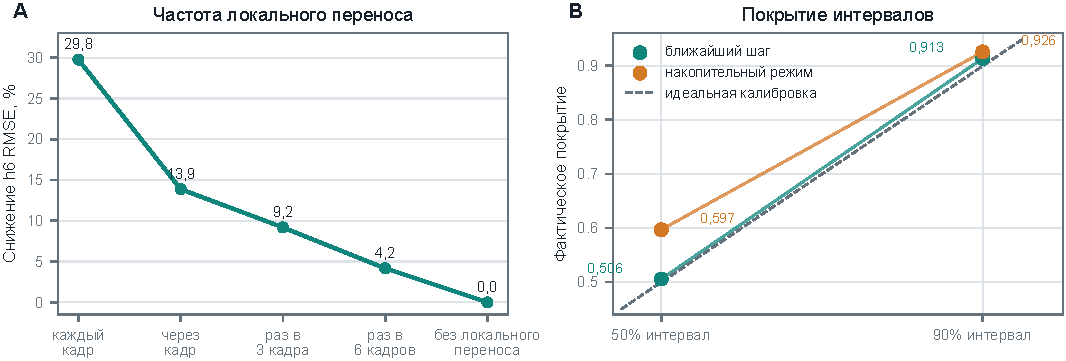
\includegraphics[width=\textwidth]{figures/fig5_robustness_calibration.pdf}
\caption{Зависимость эффекта от локального переноса и вероятностная калибровка. \textbf{A}, уменьшение h6 RMSE относительно базовой вероятностной модели без локального переноса при разной частоте поступления донорских невязок; внутреннее последовательное обновление базового фильтра во всех точках остается включенным. \textbf{B}, фактическое покрытие центральных интервалов для двух рабочих точек.}
\label{fig:robustness}
\end{figure}

\section{Методы}
\subsection{Данные и последовательный протокол}
Основной корпус LaChance содержит TrackMate-треки и временные изображения MDCK Bulk, MDCK Edge, HUVEC и MDA-MB-231 \cite{ref1}. MDCK и HUVEC снимались с интервалом 10 минут между кадрами, MDA-MB-231 - с интервалом 5 минут; поэтому последовательный h6 соответствует 60 минутам для MDCK/HUVEC и 30 минутам для MDA-MB-231. Разработческий поиск выполнялся на фиксированном разбиении фильмов MDCK Bulk 1-4/5/6. После замораживания архитектуры применялись проверка с поочередным исключением каждого из шести основных фильмов, замороженная относительно текущей конфигурации проверка на фильмах MDCK Bulk 10--16 и полная вложенная проверка с исключением фильмов HUVEC и MDA-MB-231. Фильмы 10--16 ранее участвовали в широком исследовательском просмотре, но не использовались для выбора базовой вероятностной модели, локального переноса, двух рабочих точек или их гиперпараметров. MDCK Edge использовался для оценки переноса на геометрию свободной границы.

Внешние наборы данных не объединялись с основными результатами как дополнительные успешные тесты. C2C12 с ручными и автоматическими треками использовался для проверки чувствительности к сопровождению \cite{ref22}. DeepSea проверял перенос полной последовательной системы и причинную ценность точных масок на разнородных клеточных видео \cite{ref33}. GigaScience wound healing проверял перенос коллективного поля \cite{ref23}. Синхронные измерения движения, тяги и напряжения задавали механическую верхнюю оценку \cite{ref24}. SSBD-248, S-BIAD365 и Allen использовались для проверки молекулярного, поляризационного и морфологического состояния \cite{ref25,ref26,ref27,ref28}. LifeAct-MDCK использовал три двухканальные временные последовательности для отдельной проверки формы, полярности актина, контакта и надежности \cite{ref34}. Ни один из этих межэкспериментальных переносов не прошел заранее заданный порог включения новой модальности в условное среднее ядра; LifeAct-состояние прошло только критерий добавочной информативности для масштаба ошибки. Количественные результаты приведены в дополнительном материале.

Для шести основных фильмов MDCK Bulk исходный архив временных изображений был сопоставлен с TrackMate-треками по номеру фильма, кадру и идентификатору клетки. Пространственный индекс содержал 95\,549 наблюдений клеток. Из текущих и только предшествующих кадров последовательно строились 145 многомасштабных признаков изображения, 249 признаков локального движения ткани, 215 наблюдательных признаков формы, полярности, плотности и границы, а также 401 признак нецентрированного многоклеточного окружения. После согласования доступных кадров итоговая таблица содержала 93\,596 строк и 1\,019 упорядоченных столбцов, включая ключи, координаты и показатели качества. Для каждого из шести этапов подготовки зафиксированы число строк, порядок столбцов и контрольная сумма; конвейер воспроизводит индекс клеток байт-в-байт и до начала обучения отклоняет иной порядок или состав признаков. Отбор 658 переменных для конкретного внешнего цикла выполнялся затем только по обучающим фильмам.


\begin{table}[tb]
\centering
\caption{Наборы данных и их роль. Только первые пять строк входят в количественное подтверждение итоговой архитектуры; внешние модальности использовались как заранее контролируемые проверки наблюдаемости.}
\label{tab:data}
\small
\begin{tabularx}{\textwidth}{@{}L{0.20\textwidth} L{0.25\textwidth} Y L{0.21\textwidth}@{}}
\toprule
Набор & Наблюдения & Разрез или объем & Роль \\
\midrule
MDCK Bulk 1--6 & TrackMate-треки, временные изображения & 6 внешних циклов; 81\,252 h1 и 71\,160 h6 тестовых переходов & Основное сравнение \\
MDCK Bulk 10--16 & Координатные треки & 7 фильмов, не использованных для выбора текущей конфигурации & Замороженная проверка конфигурации \\
MDCK Edge & Координатные треки, свободная граница & Замороженное транспортное ядро поверх доменной базы; 3 инициализации & Перенос оператора \\
HUVEC & Координатные треки эндотелия & 18 внешних циклов с внутридоменным обучением & Воспроизводимость архитектуры \\
MDA-MB-231 & Координатные треки опухолевых клеток & 17 внешних циклов с внутридоменным обучением & Граница в слабопредсказуемом домене \\
\midrule
C2C12 & Ручные и автоматические треки & Проверка согласованности сопровождения & Диагностика шума \\
DeepSea & Видео, маски клеток и ядер, идентификаторы & 47 видео; замороженное разбиение 26/10/11 & Частичный перенос и строгий контроль морфологии \\
LifeAct-MDCK & Два канала, маски клеток, актиновое состояние & 3 условия; непрерывные окна по 60 кадров & Внешняя проверка среднего и неопределенности \\
GigaScience wound healing & Видео и коллективное движение фронта & Исследовательский перенос & Внешняя геометрия ткани \\
Force--motion, SSBD, S-BIAD, Allen & Тяга, напряжение, молекулярное состояние, форма & 23 проверки наблюдаемости в общей матрице & Верхняя оценка модальностей \\
\bottomrule
\end{tabularx}
\end{table}

\begin{table}[tb]
\centering
\caption{Статус основных доказательств и допустимая область вывода. Разные группы фильмов не объединяются в одну парную статистику, а повторное внутридоменное обучение не называется переносом готовых весов.}
\label{tab:evidence_status}
\small
\begin{tabularx}{\textwidth}{@{}L{0.24\textwidth} L{0.22\textwidth} L{0.20\textwidth} Y@{}}
\toprule
Проверяемое утверждение & Данные и разбиение & Статус & Допустимый вывод \\
\midrule
Добавочный эффект локального переноса & MDCK Bulk 1--6, внешнее исключение фильма & Семейство H1--H2; H1: $p_{\rm Holm}=0{,}84375$, H2: $0{,}0625$ & Нулевой добавочный эффект h1 и сильный, но пограничный после поправки эффект h6 \\
Замороженная конфигурация & MDCK Bulk 10--16 & 7/7 фильмов; вторичный направленный анализ & Воспроизводимость выбранной конфигурации, но не полностью перспективное подтверждение \\
Перенос локального оператора & MDCK Edge & Замороженное ядро, доменно обученная база & Перенос коллективной поправки, а не всей модели без дообучения \\
Воспроизводимость архитектуры & HUVEC и MDA-MB-231 & Полное вложенное исключение фильма & Устойчивость процедуры обучения внутри домена; MDA остается с низким абсолютным $R^2$ \\
Новая визуальная модальность & DeepSea и LifeAct-MDCK & Частичный перенос; исследовательская проверка неопределенности & Маски не улучшают среднее; LifeAct-состояние уточняет масштаб ошибки при $n=3$ условиях \\
\bottomrule
\end{tabularx}
\end{table}

Пусть $x_{i,t}\in\mathbb R^2$ - наблюденный центроид, $d_{i,t}=x_{i,t}-x_{i,t-1}$ - завершенное смещение, а $\mathcal I_t$ - совокупность сведений, содержащая историю клетки и только те соседские переходы, которые завершились не позднее кадра $t$. Задача прогноза без обращения к будущим наблюдениям имеет вид

\begin{equation}
p_\Theta(d_{i,t+1}\mid\mathcal I_t).
\end{equation}
Прогноз перехода $t\rightarrow t+1$ сначала записывается и фиксируется. После поступления $x_{i,t+1}$ вычисляется невязка $e_{i,t+1}=d_{i,t+1}-\widehat d_{i,t+1|t}$. Она может изменить только состояние и прогнозы следующего цикла; ни сам $x_{i,t+1}$, ни производные от него признаки не входят в $\mathcal I_t$. Накопительное смещение на горизонте $H$ равно

\begin{equation}
\widehat D_{i,t}^{(H)}=\sum_{k=1}^{H}\widehat d_{i,t+k}.
\end{equation}
В отличие от фиксированного многокадрового прогноза, между слагаемыми поступают новые наблюдения. Поэтому старый оптимум среди кандидатов из одной исходной точки не является нижней границей ошибки последовательного h6.

В каждом цикле итоговая архитектура оценивает не произвольную траекторию, а условное распределение одного следующего смещения. Координатная модель сначала формирует опорный прогноз $a_{i,t}^{(1)}$. Рекуррентный фильтр выдает прямую оценку $\widetilde\mu^{\mathrm{dir}}_{i,t+1}$, а базовое условное среднее интерполирует ее с опорным прогнозом коэффициентом $\eta_{\mathrm{base}}$, выбранным только на проверочном фильме. После этого отдельный оператор рабочей точки $o$ добавляет ограниченную локальную поправку:

\begin{equation}
\begin{aligned}
\mu^{\mathrm{base}}_{i,t+1}
&=(1-\eta_{\mathrm{base}})a_{i,t}^{(1)}
+\eta_{\mathrm{base}}\widetilde\mu^{\mathrm{dir}}_{i,t+1},\\
\mu^{(o)}_{i,t+1}
&=\mu^{\mathrm{base}}_{i,t+1}
+\mathcal B_{b_o}\!\left(B_o\phi_{i,t}\right),\\
p_\Theta(d_{i,t+1}\mid\mathcal I_t)
&=\prod_{c\in\{x,y\}}
t_\nu\!\left(d_{i,t+1,c};\mu^{(o)}_{i,t+1,c},s_{i,t+1,c}\right).
\end{aligned}
\end{equation}
Здесь $\phi_{i,t}$ содержит нормализованные собственную и соседские невязки, завершенные не позднее $t$, $B_o$ является регуляризованным линейным оператором выбранной рабочей точки, а $\mathcal B_{b_o}$ ограничивает норму коллективной поправки. Опорный координатный прогноз одновременно входит в рекуррентный модуль как условие и остается в базовом среднем через интерполяцию. Масштаб $s$ и степень свободы $\nu$ наследуются от вероятностного фильтра; локальный оператор сдвигает только среднее.

\subsection{Базовый координатный прогноз}
Первая стадия формирует базовую траекторию, поэтому дальнейшие модули не начинают прогноз с нулевого вектора. Вход содержит шесть предыдущих положений трека, мгновенную и многомасштабную по времени скорость, а также табличные координатные, потоковые, морфологические и наблюдательные косвенные признаки. В основной конфигурации после объединения блоков и отбора по дисперсии только на обучающих фильмах размерность представления равна 658; состав может меняться между внешними циклами, поскольку признаки тестового фильма не участвуют в отборе. Полный словарь исходных столбцов, правила образования семейств и машинный протокол отбора приведены в дополнительном материале. Эти табличные косвенные признаки следует отличать от самостоятельных глубоких визуальных, сегментационных и механических ветвей, которые не прошли критерий добавочного сигнала и в итоговую архитектуру не вошли. Будущее не входит в набор входных данных.

На обучающих фильмах стандартизованные остаточные траектории группируются в $M=12$ классов. Для каждого класса отдельная линейная модель с $L_2$-регуляризацией предсказывает шесть последовательных остаточных смещений. Классификатор, использующий только доступные к моменту прогноза данные, оценивает $p(m\mid\mathcal I_t)$, после чего восемь наиболее вероятных моделей смешиваются с равными весами. Объединенный линейный калибратор получает эту смесь, вероятности классов, доступный контекст и выходы отдельных моделей и преобразует их в базовую траекторию

\begin{equation}
a_{i,t}^{1:6}=A_\phi(H_{i,t},V_{i,t},C_{i,t}).
\end{equation}
Здесь $H_{i,t}$ обозначает историю координат и смещений, $V_{i,t}$ - мгновенные скорости и скорости за несколько временных интервалов, а $C_{i,t}$ - локальные признаки, доступные к моменту прогноза. Метки классов траекторий и истинные остатки доступны только при обучении специализированных моделей. Опорные прогнозы для обучения последующего фильтра строятся вне выборки по фильмам, чтобы целевой фильм не участвовал в их оценке. При применении стадия выдает одну устойчивую базовую траекторию, а не выбирает лучший вариант после наблюдения цели. Ее первый шаг используется и как вход рекуррентного модуля, и как один из членов итоговой интерполяции.

\subsection{Вероятностный фильтр состояния}
Вторая стадия получает компактное состояние опорного координатного прогноза $S_{i,t}$, временную последовательность из шести доступных прошлых шагов и предыдущее скрытое состояние. Каждый элемент временной последовательности содержит предыдущую одношаговую невязку базового прогноза, наблюденную скорость и маску доступности. В $S_{i,t}$ входят шесть шагов базовой траектории, их накопительные суммы и модули, базовое и текущее смещения, нормированные положение и номер кадра. Полный исходный набор из 658 признаков используется первой стадией, но не подается повторно непосредственно в зафиксированное рекуррентное ядро. Это различие важно для правильной интерпретации абляции контекста. Рекуррентный кодировщик с размерностью 128 вычисляет

\begin{equation}
z^-_{i,t}=F_\theta(z_{i,t-1},H_{i,t},S_{i,t}).
\end{equation}
До появления следующего кадра прямой прогноз в стандартизованных координатах цели вычисляется с учетом опорного координатного прогноза,

\begin{equation}
\widetilde\mu^{\mathrm{dir,std}}_{i,t+1}
=
b_\mu\tanh\left[
\frac{W_\mu\,G_\theta(z^-_{i,t},S_{i,t},H_{i,t},a_{i,t}^{(1)})}{b_\mu}
\right],
\qquad
\widetilde\mu^{\mathrm{dir}}_{i,t+1}
=m_d+s_d\odot\widetilde\mu^{\mathrm{dir,std}}_{i,t+1},
\end{equation}
а итоговый выход интерполирует эту прямую оценку с опорным прогнозом:

\begin{equation}
\mu^{\mathrm{base}}_{i,t+1}
=(1-\eta_{\mathrm{base}})a^{(1)}_{i,t}
+\eta_{\mathrm{base}}\widetilde\mu^{\mathrm{dir}}_{i,t+1}.
\end{equation}
Здесь $m_d$ и $s_d$ оцениваются только на обучающей части, а $\eta_{\mathrm{base}}\in\{0{,}75;1\}$ выбирается на проверочном фильме. Условное распределение факторизовано по координатам:

\begin{equation}
p_{\mathrm{base}}(d_{i,t+1}\mid\mathcal I_t)
=
\prod_{c\in\{x,y\}}
t_\nu\!\left(d_{i,t+1,c};\mu^{\mathrm{base}}_{i,t+1,c},s_{i,t+1,c}\right).
\end{equation}
Величина $s$ является масштабом распределения, а не диагональной ковариацией. Степень свободы обучается и в зафиксированной контрольной точке близка к 3,89. Тяжелые хвосты уменьшают влияние редких больших смещений и ошибок сопровождения.

Фильтр отдельно оценивает положительные двухкомпонентные масштабы $q_{i,t}$ и $r_{i,t}$, обозначающие соответственно функциональную процессную и наблюдательную неопределенность. Большое $r$ соответствует менее надежному наблюдению. По одним координатным трекам квадратичная сумма $\sqrt{q_c^2+r_c^2}$ идентифицируется существенно лучше, чем каждое слагаемое по отдельности; поэтому они не трактуются как прямые физические оценки двух видов шума. Усредненное по компонентам аналитическое усиление имеет вид

\begin{equation}
K^0_{i,t}
=\frac{1}{2}\sum_{c\in\{x,y\}}
\frac{q^2_{i,t,c}}{q^2_{i,t,c}+r^2_{i,t,c}}.
\end{equation}
Нейронная поправка к его логиту зависит от предварительного состояния, статического кодирования и нормированной невязки:

\begin{equation}
K_{i,t}=\operatorname{sigmoid}
\left[
\operatorname{logit}(K^0_{i,t})
+\Delta K_\theta\left(
z^-_{i,t},E_\theta(S_{i,t}),
\frac{e_{i,t}}{\sqrt{q^2_{i,t}+r^2_{i,t}}},
\log q_{i,t},\log r_{i,t},m_{i,t}
\right)
\right].
\end{equation}
После наблюдения состояние обновляется по

\begin{equation}
z_{i,t}=\operatorname{Norm}
\left[
z^-_{i,t}+m_{i,t}K_{i,t}\odot
U_\theta(e_{i,t},q_{i,t},r_{i,t})
\right],
\end{equation}
где $m_{i,t}=0$ при пропущенном наблюдении. На обучении случайно скрывались 15\% наблюдений и добавлялся координатный шум 0,35 пикселя. Граф не входит в обязательное рекуррентное ядро, поскольку его раннее включение не давало преимущества над перемешанным соседством.

\subsection{Локальный перенос невязок}
Третья стадия использует только завершенные ошибки. Сначала физическая невязка каждой координаты преобразуется в нормальную оценку

\begin{equation}
z_{i,t,c}
=
\Phi^{-1}\!\left[
F_{t_\nu}\!\left(
\frac{d_{i,t,c}-\mu^{\mathrm{base}}_{i,t,c}}{s_{i,t,c}}
\right)
\right].
\end{equation}
Для пространственных масштабов 30, 60, 120 и 240 пикселей вычисляется

\begin{equation}
\overline z_{i,t}^{(\ell)}=
\frac{\sum_{j\ne i}w_{ij,t}^{(\ell)}z^{done}_{j,t}}
{\sum_{j\ne i}w_{ij,t}^{(\ell)}},
\qquad
w_{ij,t}^{(\ell)}=
\exp\left[
-\frac{\|x_{i,t}-x_{j,t-1}\|^2}{2\ell^2}
\right]
\mathbb I\!\left(\|x_{i,t}-x_{j,t-1}\|\le R\right).
\end{equation}
Позиция донора относится к кадру выпуска уже завершенного перехода; собственная траектория исключается только из соседских средних, но собственная предыдущая оценка $z$ остается отдельным входом. В подтвержденной Bulk-реализации

\begin{equation}
R_{t}=4\,\xi_{\mathrm{train}}\,d_{\mathrm{nn},t},
\end{equation}

где $\xi_{\mathrm{train}}$ является медианой экспоненциальных длин в единицах расстояния до ближайшего соседа, оцененных только по обучающим фильмам внешнего цикла, а $d_{\mathrm{nn},t}$ -- медианный масштаб ближайшего соседства текущего кадра. Гауссовы масштабы $\ell\in\{30,60,120,240\}$ остаются заданными в пикселях. Отдельная внешняя проверка HUVEC/MDA-MB-231 использовала непараметрическое пересечение $e^{-1}$ в пикселях, оцененное только на обучающих данных, и является исследовательской, а не частью подтвержденной Bulk-спецификации.

До взаимодействия с прогнозным масштабом набор содержит 25 величин: собственные $z_x,z_y$, их доступность, средние $z_x,z_y$ по кадру и для каждого из четырех пространственных масштабов локальные средние, покомпонентные стандартные отклонения и эффективное число соседей. Итоговый набор признаков

\begin{equation}
\phi=[u,\ u\,s_x^{\mathrm{base}},\ u\,s_y^{\mathrm{base}}]\in\mathbb R^{75}
\end{equation}

добавляет взаимодействия всего набора $u$ с двумя компонентами прогнозного масштаба базового прогноза. Таким образом, локальный оператор получает стандартизованную вероятность ошибки и ее ожидаемую физическую амплитуду, не смешивая их неявно.

Регуляризованный линейный оператор $B_o$ дает сырую поправку $\widetilde c^{(o)}_{i,t+1}=B_o\phi_{i,t}$. Ее норма ограничивается гладко:

\begin{equation}
c^{(o)}_{i,t+1}=
b_o\tanh\left(\frac{\|\widetilde c^{(o)}_{i,t+1}\|}{b_o}\right)
\frac{\widetilde c^{(o)}_{i,t+1}}
{\max(\|\widetilde c^{(o)}_{i,t+1}\|,\varepsilon)}.
\end{equation}
Итоговое среднее в развернутом виде равно


\begin{table}[tb]
\centering
\caption{Замороженная спецификация итоговой архитектуры.}
\label{tab:architecture}
\small
\begin{tabularx}{\textwidth}{@{}L{0.23\textwidth} Y@{}}
\toprule
Компонент & Реализация и ограничение \\
\midrule
Опорный координатный прогноз & 6 предыдущих положений, мгновенная скорость и скорости за несколько интервалов, доступный контекст; 12 моделей классов остаточных траекторий, равная смесь 8 наиболее вероятных и объединенный линейный калибратор с $L_2$-регуляризацией; вневыборочные по фильмам обучающие опорные прогнозы. \\
Фильтр состояния & Рекуррентное скрытое состояние 128; история предыдущих невязок, скоростей и доступности; двухкомпонентные функциональные масштабы процессной и наблюдательной ошибки; обучаемая поправка к усилению. \\
Вероятностный выход & Произведение двух одномерных распределений Стьюдента; обучаемые масштабы и степень свободы; итоговая интерполяция с опорным координатным прогнозом. \\
Граф взаимодействия & Нормальные оценки только завершенных невязок; гауссовы веса на масштабах 30, 60, 120 и 240 px внутри опоры $R_t=4\xi_{\mathrm{train}}d_{\mathrm{nn},t}$, оцененной только на обучающих фильмах; собственная клетка исключена из соседских средних. \\
Калибратор & Для каждой рабочей точки $o$ отдельно оцениваются $B_o$, регуляризация $\alpha_o$ и ограничение нормы $b_o$; локальная ветвь сдвигает только среднее. \\
Обучение & Хронологические фрагменты; усечение 8 кадров; до 32 эпох; 15\% пропусков; шум координат 0,35 px; три инициализации. \\
Размер & 380\,553 параметра рекуррентного ядра, около 1,54 МБ; радиусный поиск имеет измеренную почти линейную зависимость от числа клеток. \\
\bottomrule
\end{tabularx}
\end{table}

\begin{equation}
\mu^{(o)}_{i,t+1}
=
\mu^{\mathrm{base}}_{i,t+1}
+\mathcal B_{b_o}\!\left(B_o\phi_{i,t}\right).
\end{equation}
Первое слагаемое является базовым условным средним, объединяющим прямой выход рекуррентного модуля, опорный координатный прогноз и индивидуальную память. Второе добавляет только ту часть локального остатка, которую допускает ограничение нормы. Режим ближайшего шага и накопительный режим используют одинаковые опорный прогноз, $F_\theta$ и $U_\theta$, но разные веса горизонтов, $B_o$, $\alpha_o$ и $b_o$, выбранные только по внутреннему проверочному фильму. Линейность последнего оператора является намеренным ограничением: коллективная часть остается проверяемой и не получает свободную глубокую параметризацию после широкого архитектурного поиска.

\subsection{Полевой закон и механический контроль}
Дополнительная полевая проверка использовала 22 островка MDCK из набора одновременных измерений движения, тяги к субстрату и напряжения монослоя \cite{ref24}. Единицей внешнего исключения был островок. Для каждого тестового островка один другой целый островок той же экспериментальной группы использовался для выбора регуляризации, а остальные -- для оценки коэффициентов. Таблица содержала 105\,890 причинно выровненных полевых точек. Скорость перехода $t\rightarrow t+1$ была целью; вход движения заканчивался завершенным переходом $t-1\rightarrow t$. Тяга и напряжение относились к кадру выпуска $t$. Поля будущей механики сохранялись в исходном техническом наборе только для прежних верхних оценок и были программно исключены из причинной библиотеки.

Пространственные производные вычислялись на исходной прямоугольной сетке с шагом 7,92 $\mu$m, после чего оценка бралась в каждой шестой точке внутри наблюдаемого островка. Таким образом, прореживание влияло на число статистических точек, но не на конечно-разностный оператор. В библиотеку входили $u$, $\nabla^2u$, $\nabla(\nabla\!\cdot u)$, $(v\!\cdot\nabla)u$, $(u\!\cdot\nabla)u$, $\|u\|^2u$ и нормаль границы с экспоненциальным затуханием. Привилегированная механическая версия добавляла векторы тяги, дивергенции напряжения и их баланса. Для каждой векторной функции обучался один скалярный коэффициент, общий для обеих координат, без векторного свободного члена. Масштаб каждого члена определялся одной среднеквадратичной нормой по двум компонентам на обучающих островках; редкие выбросы ограничивались по модулю вектора, а не покомпонентно.

Коэффициенты оценивались гребневой регрессией для $\alpha\in\{0{,}01;0{,}1;1;10;100\}$ с последующим исключением членов ниже 0, 1 или 3\% наибольшего стандартизованного коэффициента и повторной оценкой оставшейся опоры. Настройка проводилась только на проверочном островке. Нулевые контроли сдвигали поле на один доступный момент при сохранении координаты, циклически сдвигали его внутри кадра или подставляли другой островок; те же операции отдельно применялись к измеренной механике.

Для проверки потенциальной интерпретации отдельно оценивался градиентный сектор $\{u,\nabla^2u,\nabla(\nabla\!\cdot u),\|u\|^2u\}$ без адвекции. Знаково ограниченная гребневая регрессия требовала $a<1$ для коэффициента прямой памяти, неотрицательных коэффициентов при лапласиане и градиенте дивергенции и неположительного коэффициента при кубическом члене; это эквивалентно условиям $r=1-a>0$, $K_T\geq0$, $K_L\geq0$ и $g\geq0$ в уравнении~\eqref{eq:effective_functional}. Регуляризация выбиралась на целом проверочном островке из того же набора значений, после чего модель повторно оценивалась на обучающих и проверочном островках. Свободная, ограниченная, дополненная границей и полная адвективная версии сравнивались на одном наборе внешних островков.

Согласованность с диссипативным направлением сначала оценивалась диагностикой первого порядка. Для предсказанного изменения $\delta u_{\mathrm{pred}}=\widehat u_t-u_{t-1}$ и наблюдаемого изменения $\delta u_{\mathrm{obs}}=u_t-u_{t-1}$ использовалась величина
\begin{equation}
\Delta\mathcal F_{\mathrm{eff}}^{(1)}
=-\left\langle\delta u_{\mathrm{pred}},\delta u_{\mathrm{obs}}\right\rangle .
\end{equation}
При чистом градиентном потоке отрицательный знак соответствует движению вдоль локального спуска функционала. Нулевой контроль переставлял $\delta u_{\mathrm{obs}}$ внутри внешнего островка. Для конечной проверки функционал из уравнения~\eqref{eq:effective_functional} вычислялся до и после полного обновления на исходной сетке. Сравнивались наблюдаемый переход, временная перестановка и потенциальная карта; коэффициент затухания карты выбирался только на отдельном проверочном островке. Для шестишагового развертывания каждое следующее поле строилось из предыдущего предсказанного поля, а геометрия границы фиксировалась в момент выпуска. Таким образом, ни конечная разность функционала, ни h2--h6 не используют будущую границу тестового островка.

E(2)-эквивариантное приближение LaChance оценивался отдельно от непрерывного полевого закона. Для каждого внешнего фильма строились векторные функции собственной и средней невязки, продольные и поперечные проекции соседских невязок на трех масштабах, кубическое насыщение и две адвекции. Один скалярный коэффициент каждой функции применялся к обеим координатам; свободный член отсутствовал. Потенциальная версия запрещала адвекцию и ограничивала знаки коэффициентов. Регуляризация и ограничение нормы выбирались только на внутреннем проверочном фильме. Для замороженной проверки фильмов 10--16 вся сетка параметров оценивалась перекрестно только внутри фильмов 1--6, после чего закон один раз переоценивался на всех шести разработческих фильмах. Контроли сохраняли распределение амплитуд, но подменяли клеточную идентичность или использовали более раннее завершенное время.

Вероятностная проверка использовала те же средние и исходные масштабы для гауссова и Стьюдентова семейств. Для каждого внешнего фильма множитель масштаба и радиусы конформных областей оценивались только по пяти остальным фильмам. Сообщались совместное отрицательное логарифмическое правдоподобие, энергетическая оценка, покомпонентное и радиальное покрытие 50/90\%. Для h6 масштаб калибровался непосредственно по накопительной ошибке; это проверяемое вероятностное приближение, а не предположение о независимости шести одношаговых ошибок.

В обратной механической задаче тяга, дивергенция напряжения и их баланс прогнозировались сначала по скорости, ее лапласиану, продольно-поперечному члену и границе, затем с добавлением завершенной невязки и ее производных. Перенос между условиями включал низкую/высокую плотность, контроль/обработку CytoD и раннюю/позднюю группу CN03. Продольный и поперечный динамические спектры вычислялись трехмерным преобразованием Фурье по времени и двум пространственным координатам внутри каждого исключенного островка; сообщалась ошибка логарифмической мощности. Синтетическая проверка использовала 36 независимых гладких векторных полей, шесть известных ненулевых коэффициентов, шум Стьюдента и 300 повторных выборок целых кадров. Алгебраическая эквивариантность проверялась произвольным поворотом векторных членов, сеточная -- поворотом всей конечно-разностной библиотеки на $180^\circ$.

\subsection{Свойства локального оператора}
Причинность следует из порядка вычислений: в $\phi_{i,t}$ входят только прогнозы, записанные до кадра $t$, и ошибки переходов, уже завершенных к этому кадру. Автоматическая проверка индексов подтверждает для каждого ребра, что время донорской невязки не превосходит время выпуска нового прогноза.

Гауссовы веса и радиусная опора зависят только от разности положений, поэтому геометрическое усреднение инвариантно к общему переносу координат. Если векторные входы уже заданы и поворачиваются совместно с координатами, их среднее эквивариантно: при ортогональном преобразовании $Q$ выполняется $\overline z(Qx,Qz)=Q\overline z(x,z)$. Эти два свойства геометрического подоператора подтверждены численными тестами с точностью $2\cdot10^{-12}$. Однако покомпонентное преобразование в нормальные оценки, покомпонентные дисперсии, опорный координатный прогноз и $B_o$ не обязаны коммутировать с произвольным поворотом. Поэтому строгая вращательная эквивариантность полной модели и итоговой модели не заявляется.

Ограничитель дает непосредственную оценку устойчивости
\begin{equation}
\|\mu^{(o)}_{i,t+1}-\mu^{\mathrm{base}}_{i,t+1}\|\le b_o.
\end{equation}
Если нормы донорских векторных оценок ограничены величиной $M$, а удаленная нормированная масса плотного ядра равна $\tau_R$, то для его нормированного среднего
\begin{equation}
\|m_{\mathrm{dense}}-m_{\mathrm{sparse}}\|\le 2M\tau_R.
\end{equation}
Эта граница была проверена после диагностического ограничения 99,5-го процентиля и выполнялась для всех проверенных кадров. Она является консервативной оценкой ошибки одного среднего, а не гарантией равенства конечного прогноза после повторного обучения. Построение дерева соседства требует $O(N\log N)$ операций, а применение оператора -- $O(E)$, где $E$ является числом ребер внутри опоры.

\subsection{Обучение, сравнения и статистика}
Базовый координатный модуль обучался первым и затем замораживался. Последовательный фильтр обучался на хронологических фрагментах целых треков, а не на независимо перемешанных строках. Для последовательности длины $T$ использовалась составная функция потерь

\begin{equation}
\begin{aligned}
\mathcal L={}&
\lambda_{\mathrm H}\sum_{t=1}^{T}
\operatorname{Huber}(\widehat d_{t+1},d_{t+1})
+\lambda_{\mathrm T}\sum_{t=1}^{T}
\big[-\log p_{\mathrm{StudentT}}(d_{t+1}\mid\mathcal I_t)\big]\\
&+\sum_{H\in\{2,4,6\}}\lambda_H
\operatorname{Huber}(\widehat D^{(H)},D^{(H)})
+\lambda_e\mathcal L_{e}
+\lambda_R\mathcal R(q,r,K).
\end{aligned}
\end{equation}
Первый член отвечает за устойчивое среднее следующего шага, второй - за вероятностный масштаб и тяжелые хвосты, третий ограничивает накопление ошибки, а два последних предотвращают вырожденную параметризацию функциональных масштабов $q$, $r$ и усиления. Они не делают разложение шума физически идентифицируемым. Зафиксированная конфигурация использует скрытую размерность 128, усечение обратного распространения на восьми кадрах, не более 32 эпох, скорость обучения $5\cdot10^{-4}$, штраф весов $2\cdot10^{-4}$ и долю случайно отключаемых связей 0,06.

В основной последовательной таблице сравнивались постоянная скорость, фильтры постоянной скорости и ускорения, взаимодействующая смесь кинематических моделей, устойчивый к выбросам WoLF-IMQ, GRU, градиентный бустинг и KalmanNet \cite{ref6,ref7}. Отдельный разработческий поиск включал линейную модель с $L_2$-регуляризацией, многослойный перцептрон, LSTM, Transformer и адаптированные графовые сети; он проверял архитектурные семейства, но не использовался для количественного вывода о превосходстве на замороженных фильмах. Архитектуры прогноза из одной начальной точки рассматривались еще одним отдельным уровнем, поскольку их ADE/FDE, горизонт и доступная информация не совпадают с последовательным обновлением. Для каждой строки завершающего сравнения сохранялись источник прогноза, степень соответствия исходной архитектуре, контрольная сумма упорядоченных ключей и спецификация протокола. На фильмах 10--16 GRU, HGBDT и KalmanNet обучались на фильмах 1--4 и выбирались только по фильму 5; для всех методов три инициализации объединялись усреднением прогнозов до вычисления фильмовых метрик. Вариант CV/CA KalmanNet также выбирался по фильму 5, а не по тестовой ошибке. HGBDT использовал только причинно доступные трековые признаки, общие для обеих групп фильмов.

Компонентная RMSE сначала вычислялась отдельно для каждого фильма $m$, а затем макроусреднялась:

\begin{equation}
\operatorname{RMSE}_m=
\sqrt{\frac{1}{2N_m}\sum_{n=1}^{N_m}
\|\widehat D_{m,n}-D_{m,n}\|^2_2},
\qquad
\operatorname{RMSE}_{\mathrm{macro}}
=\frac{1}{M}\sum_{m=1}^{M}\operatorname{RMSE}_m.
\end{equation}
Основное фильмовой $R^2$ вычислялось по суммарной квадратичной ошибке двумерного вектора после раздельного центрирования его координат, а затем макроусреднялось по фильмам. Поэтому приведенное в основной таблице значение 0,507733 округлено до 0,508. Для диагностического сопоставления с компонентной RMSE использовалась согласованная покомпонентная версия $R^2$: сначала $R^2$ вычислялось отдельно для двух координат, затем усреднялось; для режима ближайшего шага она равна 0,506282. Величина $s_{m,h}=\operatorname{RMSE}_{m,h}/\sqrt{1-R^2_{m,h}}$ вычислялась именно с этой покомпонентной мерой отдельно внутри каждого фильма и только затем усреднялась; она использовалась как тождественно восстановленный разброс цели, а не как оценка неприводимой дисперсии шума. Дополнительно оценивались косинус направления, отношение модулей, отрицательное логарифмическое правдоподобие и покрытие интервалов.

Для проверки компромисса h1--h6 до запуска была задана сетка $\lambda=0,0{,}1,\ldots,1$. Веса горизонтов линейно интерполировались между $(0{,}80,0{,}10,0{,}06,0{,}04)$ и $(0{,}10,0{,}10,0{,}20,0{,}60)$ для h1, h2, h4 и h6; допустимое ухудшение h1 на проверочном фильме одновременно возрастало от 0,5 до 10\%. Для каждой внешней итерации коэффициент $L_2$-регуляризации и граница поправки выбирались на одном внутреннем проверочном фильме, после чего модель переобучалась на обучающих и проверочном фильмах и один раз оценивалась на исключенном фильме. В замороженное статистическое семейство выпуска вошли только крайние рабочие точки: H1 для $\lambda=0$ на h1 и H2 для $\lambda=1$ на h6. Промежуточные точки используются только для описания геометрии фронта. Группа фильмов 1--6 остается разработческой по истории проекта, тогда как фильмы 10--16 дают отдельную проверку уже зафиксированной конфигурации.

Статистической единицей был фильм, а не клетка или отдельный переход. Парные различия проверялись точным двусторонним тестом со сменой знака всех $2^M$ наборов фильмовых разностей и бутстрепом фильмов. Основное семейство состояло ровно из двух гипотез: H1 сравнивала режим ближайшего шага с базовой вероятностной моделью на h1, H2 -- накопительный режим с той же моделью на h6. Их двусторонние значения корректировались ступенчатой процедурой Холма; все остальные сочетания метода и горизонта считались описательными или исследовательскими. Отдельный односторонний анализ четырех горизонтов на фильмах 10--16 сообщался как вторичный и не объединялся с H1--H2. Для основных прогностических интервалов использовалось 20\,000 повторных выборок фильмов, для диагностических кривых поля -- 2\,000, а для завершающих парных сравнений обучаемых методов на семи фильмах -- 100\,000; сообщались процентильные 95\% интервалы. Эти процедуры не требуют предположения о нормальности клеточных ошибок. Порог значимости был равен 0,05. При шести фильмах минимальное двустороннее значение точного теста равно 0,03125, при семи -- 0,015625. Переходы не исключались по величине прогностической ошибки; включение определялось только заранее заданной доступностью истории и непрерывностью честных последовательных выпусков. Расчет выполнялся в Python 3.11.9 с NumPy 2.0.2, pandas 2.2.3, SciPy 1.17.1, scikit-learn 1.8.0 и PyTorch 2.8.0.

\section{Обсуждение}
Предлагаемая архитектура работает не потому, что восстанавливает универсальный закон взаимодействия из статической конфигурации. Она разделяет три уровня информации. Опорный координатный прогноз сообщает фильтру устойчивую индивидуальную динамику; вероятностный фильтр непосредственно оценивает следующий шаг и обновляет память клетки по собственной завершенной невязке; локальный оператор переносит кратковременно согласованную часть уже реализованного возмущения соседей. Благодаря такому порядку граф получает измеренный динамический сигнал, а не должен извлекать направление из одной геометрии.

Физическая интерпретация относится к огрубленной кинематике, а не к прямой механике. Невязка может содержать изменение поляризации, локальное ускорение ткани, контактное событие, ненаблюдаемое механическое поле, ошибку модели и ошибку центроида. По одним трекам эти причины неразделимы. Данные непосредственно подтверждают пространственную согласованность, ее уменьшение с расстоянием и необходимость правильного времени и идентичности. Поэтому графовую поправку можно интерпретировать только как кратковременную приближенную кинематическую оценку коллективного возмущения, условную по ошибкам базового прогноза. Называть ее скоростью ткани, силой, давлением или тягой нельзя без одновременных механических измерений и установленного соотношения сила-скорость.

Внешняя E(2)-эквивариантная проверка уточняет эту границу. Устойчивые знаки лапласиана, продольно-поперечного члена, адвекции и кубического насыщения и провал пространственно-временных подмен подтверждают, что завершенная невязка имеет нетривиальную полевую динамику. Прямой перенос на LaChance устраняет прежний разрыв между этой проверкой и итоговым графом: ограниченный потенциальный закон объясняет 95,1\% дисперсии полезной накопительной поправки и сохраняет 96,5\% ее выигрыша, а на замороженных фильмах проходит временной и идентификационный контроли. Следовательно, сходство двух представлений является измеренным свойством архитектуры, а не только качественной аналогией.

Потенциальное разложение одновременно задает строгую границу физической трактовки. Почти весь прогностический выигрыш полного полевого закона содержится в секторе релаксации, пространственного сглаживания, продольно-поперечного перераспределения и нелинейного насыщения; адвективный сектор добавляет малую поправку. Потенциальная карта устойчива при конечном шестишаговом развертывании и монотонно уменьшает собственный функционал, что согласуется с представлением ``градиентный поток плюс активный перенос'' \cite{ref2,ref32}. Однако наблюдаемые переходы не уменьшают этот функционал чаще временной перестановки, а тяга и напряжение не улучшают прогноз даже при интервенционном переносе. Поэтому работа получила интерпретируемый кинематический оператор и ляпуновоподобный функционал его потенциальной части, но не восстановила гидродинамическое уравнение или запасенную энергию ткани. Для такого утверждения потребовались бы воспроизводимая связь с одновременной механикой, предсказание нового вмешательства и преимущество над нулевыми контролями в наблюдаемой конечной динамике.

Отрицательные ветви являются частью доказательства, а не перечнем неудач. $c(r)$ не сохраняет ориентацию и историю контакта; условный $C(1,2)$ теоретически богаче, но проверенные состояния не сделали его направленным и прогностически доступным. Генератор кандидатов увеличивал покрытие, но не наблюдаемость режима. Учитель с будущим показывал существование разделимых траекторных классов, но ученик, получавший только прошлое, не восстанавливал их. Видео, маски и механика не прошли строгие контроли переноса для условного среднего. LifeAct-состояние уточнило границу: оно улучшило оценку вероятностного масштаба, но не направление следующего шага. На этом фоне локальная завершенная невязка осталась единственным коллективным сигналом, одновременно выдержавшим пространственную, временную и идентификационную проверку как поправка среднего.

Метод занимает промежуточное место между прогнозированием траекторий и последовательным усвоением наблюдений. В отличие от AgentFormer, MTR и QCNet, он не строит фиксированную многорежимную сцену на несколько кадров вперед. В отличие от классического фильтра Калмана, усиление и распределение с тяжелыми хвостами зависят от истории клетки. В отличие от обычной графовой сети, соседское сообщение появляется только после наблюдения завершенного перехода. Научный вклад поэтому состоит в строго последовательном интерфейсе между индивидуальным прогнозом и локальным полем невязки, а не в новой универсальной графовой ячейке.

Существуют девять существенных ограничений. Во-первых, h6 является накоплением шести последовательных прогнозов с промежуточными наблюдениями, а не предвидением шести кадров из одной точки. Во-вторых, улучшение h1 относительно сильного базового прогноза не подтверждено, а накопительный режим сознательно ухудшает ближайший шаг; в завершающей семифильмовой проверке GRU имела меньшую h1 RMSE. Малый масштаб h1-цели и конечная ошибка локализации объясняют, почему его $R^2$ ниже, чем на h6, но не отменяют эту отрицательную сравнительную проверку. В-третьих, абсолютная предсказуемость MDA-MB-231 остается низкой, несмотря на устойчивый относительный эффект. В-четвертых, пространственная длина корреляции зависит от домена и способа ее определения: близкий пиксельный масштаб в двух сериях MDCK Bulk не образует универсального безразмерного закона, а экспоненциальная аппроксимация нестабильна на части внешних фильмов. Фиксированная пиксельная опора не прошла допуск 0,2\%, тогда как адаптивная опора через $d_{\mathrm{nn},t}$ прошла его. В-пятых, синтетический стенд правильно восстанавливает точечные параметры поля, но пока не обеспечивает надежного интервального покрытия для анизотропии. В-шестых, основная шестифильмовая таблица не полностью унифицирована по правилу объединения инициализаций: базовые нейронные модели представлены средним метрик, а итоговая модель использует заранее заданный ансамбль трех прогнозов. Завершающая таблица на фильмах 10--16 устраняет эту асимметрию для GRU, HGBDT и KalmanNet путем усреднения прогнозов до расчета метрик, но сама эта группа не является полностью гипотезно-наивной. В-седьмых, E(2)-эквивариантность доказана для ограниченной альтернативной библиотеки, а не для всего итогового предиктора: опорный координатный прогноз и свободный 75-признаковый калибратор ей не обязаны. Ограниченный закон немного уступает лучшей плотной поправке на замороженной h6-проверке (4,842 против 4,820 пикселя), поэтому остается интерпретируемой приближенной моделью. В-восьмых, монотонное уменьшение $\mathcal F_{\mathrm{eff}}$ относится к потенциальной карте модели; наблюдаемая ткань не превзошла временную перестановку, а перенос механической модальности не прошел контроль. В-девятых, проверка LifeAct содержит только три независимых условия, использует автоматически построенные треки, а одна последовательность имеет погранично высокое покрытие маской; поэтому его положительный результат по NLL является исследовательским и не доказывает перенос на LaChance. Эти ограничения не меняют прогностического результата, но запрещают трактовать оператор как универсальную механику, функционал как физическую энергию или малое различие h1 как преимущество архитектуры.

Квадратичная исследовательская реализация не является обязательной частью метода. Радиусный оператор с опорой $R=4\xi$ прошел заранее заданный односторонний допуск неухудшения 0,2\% по точечным оценкам h1 и h6, сохранил временные и идентификационные контроли и использовал в среднем 38,3\% плотных ребер. Это инженерный критерий сохранения качества, а не статистический тест эквивалентности. Эмпирическая сложность оператора была близка к линейной по числу клеток после построения дерева соседства. Рекуррентное ядро содержит 380 553 параметра и занимает около 1,54 МБ, но компактность ядра не следует смешивать со стоимостью предварительного построения координатного контекста.

Текущие данные позволяют заявлять наименьшую h6 RMSE среди завершенных согласованных базовых методов из таблицы~\ref{tab:benchmark}. Они не позволяют заявлять глобальное превосходство для всех задач клеточного движения, поскольку общепринятого последовательного эталона с тем же порядком наблюдений пока нет, часть внешних современных архитектур использует другой набор доступной информации, а правило объединения инициализаций еще не унифицировано для всех нейронных сравнений.

\section{Заключение}
Систематический архитектурный поиск показал, что основным ограничением прогноза клеточного движения является не отсутствие геометрически правдоподобного будущего, а недостаточная возможность заранее определить реализующийся режим. Статическая физика, свободное графовое сообщение, широкие генераторы и прямые дополнительные модальности не закрыли этот разрыв. Перевод задачи в последовательный протокол сделал доступным другой источник информации: локально согласованную ошибку уже завершенного движения.

Итоговая модель сочетает базовый координатный прогноз, фильтр состояния с тяжелохвостым распределением и ограниченный многомасштабный перенос невязок. Она сохраняет сильное качество ближайшего шага и существенно уменьшает накопительную ошибку при регулярном поступлении наблюдений. Радиусная реализация воспроизводит плотный оператор в пределах заданного допуска, а внешняя по фильму калибровка подтверждает вероятностные оценки. Отдельный E(2)-эквивариантный потенциальный закон воспроизводит основную часть полезной графовой поправки как на разработческих, так и на замороженных фильмах; конечный полевой опыт подтверждает устойчивость этого закона, но не физическую энергетическую трактовку. Пространственное затухание сигнала, контроли времени и идентичности, перенос транспортного ядра в MDCK Edge и воспроизведение архитектурного эффекта после внутридоменного обучения HUVEC/MDA-MB-231 образуют согласованное, но не универсальное доказательство метода. Работа тем самым предлагает не окончательную механическую модель миграции, а воспроизводимый способ использовать условно предсказуемую коллективную компоненту невязки там, где скрытое состояние невозможно надежно восстановить заранее.

\section*{Доступность данных}
Основной корпус LaChance доступен в Zenodo, запись 4959169 (\url{https://doi.org/10.5281/zenodo.4959169}); остальные открытые наборы и их постоянные идентификаторы приведены в соответствующих ссылках. Реализация LIT-Cell, договоры данных, словарь 1\,019 исходных столбцов, контрольные суммы промежуточных таблиц и команды полного воспроизведения доступны по адресу \url{https://github.com/dmitriy5143/lit-cell}. Дополнительный материал содержит матрицу архитектурного поиска, конфигурации моделей, отрицательные результаты и проверку разреженного оператора.

\section*{Подписи к дополнительным материалам}
\noindent\textbf{S1 Text. Полный доказательный и воспроизводимый протокол.}
Матрица архитектурного поиска, сопоставимые базовые методы, парная статистика, внешние проверки, замороженная конфигурация, характеристика поля невязок, синтетическая верификация и договор причинного воспроизведения.

\begingroup
\footnotesize\setstretch{1.0}
\begin{thebibliography}{34}
\setlength{\itemsep}{1pt}
\setlength{\parsep}{0pt}
\bibitem{ref1} J. LaChance, K. Suh, J. Clausen, and D. J. Cohen, “Learning the rules of collective cell migration using deep attention networks,” \textit{PLoS Computational Biology}, vol. 18, no. 4, e1009293, 2022. \url{https://doi.org/10.1371/journal.pcbi.1009293}

\bibitem{ref2} R. Alert and X. Trepat, “Physical models of collective cell migration,” \textit{Annual Review of Condensed Matter Physics}, vol. 11, pp. 77-101, 2020. \url{https://doi.org/10.1146/annurev-conmatphys-031218-013516}

\bibitem{ref3} X. Trepat et al., “Physical forces during collective cell migration,” \textit{Nature Physics}, vol. 5, pp. 426-430, 2009. \url{https://doi.org/10.1038/nphys1269}

\bibitem{ref4} L. Rossetti et al., “Optogenetic generation of leader cells reveals a force-velocity relation for collective cell migration,” \textit{Nature Physics}, vol. 20, pp. 1659-1669, 2024. \url{https://doi.org/10.1038/s41567-024-02600-2}

\bibitem{ref5} H. Yang et al., “Learning collective cell migratory dynamics from a static snapshot with graph neural networks,” \textit{PRX Life}, vol. 2, 043010, 2024. \url{https://doi.org/10.1103/PRXLife.2.043010}

\bibitem{ref6} G. Revach et al., “KalmanNet: Neural network aided Kalman filtering for partially known dynamics,” arXiv:2107.10043, 2021. \url{https://arxiv.org/abs/2107.10043}

\bibitem{ref7} M. Roth, T. Ardeshiri, E. Ozkan, and F. Gustafsson, “Robust Bayesian filtering and smoothing using Student's t distribution,” arXiv:1703.02428, 2017. \url{https://arxiv.org/abs/1703.02428}

\bibitem{ref8} Y. Yuan, X. Weng, Y. Ou, and K. Kitani, “AgentFormer: Agent-aware transformers for socio-temporal multi-agent forecasting,” in \textit{Proc. ICCV}, pp. 9813-9823, 2021.

\bibitem{ref9} S. Shi, L. Jiang, D. Dai, and B. Schiele, “Motion Transformer with global intention localization and local movement refinement,” in \textit{Advances in Neural Information Processing Systems}, vol. 35, pp. 6531-6543, 2022.

\bibitem{ref10} Z. Zhou, J. Wang, Y.-H. Li, and Y.-K. Huang, “Query-centric trajectory prediction,” in \textit{Proc. CVPR}, pp. 17863-17873, 2023.

\bibitem{ref11} A. Prutsch, D. Schinagl, and H. Possegger, “Streaming real-time trajectory prediction using endpoint-aware modeling,” in \textit{Proc. WACV}, pp. 3005--3014, 2026. \href{https://openaccess.thecvf.com/content/WACV2026/html/Prutsch_Streaming_Real-Time_Trajectory_Prediction_Using_Endpoint-Aware_Modeling_WACV_2026_paper.html}{Страница публикации}.

\bibitem{ref12} A. Prutsch, C. Fruhwirth-Reisinger, D. Schinagl, and H. Possegger, “SHARP: Short-window streaming for accurate and robust prediction in motion forecasting,” in \textit{Proc. CVPR}, pp. 32103--32112, 2026. \href{https://openaccess.thecvf.com/content/CVPR2026/html/Prutsch_SHARP_Short-Window_Streaming_for_Accurate_and_Robust_Prediction_in_Motion_CVPR_2026_paper.html}{Страница публикации}.

\bibitem{ref13} I. Bae, J. Oh, and H.-G. Jeon, “EigenTrajectory: Low-rank descriptors for multi-modal trajectory forecasting,” arXiv:2307.09306, 2023.

\bibitem{ref14} Y. Song et al., “Score-based generative modeling through stochastic differential equations,” arXiv:2011.13456, 2020.

\bibitem{ref15} M. C. Comes et al., “Accelerating the experimental responses on cell behaviors: A long-term prediction of cell trajectories using Social Generative Adversarial Network,” \textit{Scientific Reports}, vol. 10, 15635, 2020.

\bibitem{ref16} R. Pradeep et al., “Contrastive learning of cell state dynamics in response to perturbations,” arXiv:2410.11281, 2024.

\bibitem{ref17} B. Gallusser, M. Stieber, and M. Weigert, “Self-supervised dense representation learning for live-cell microscopy with time arrow prediction,” in \textit{Proc. MICCAI}, 2023.

\bibitem{ref18} M. C. Robitaille et al., “Self-supervised machine learning for live cell imagery segmentation,” \textit{Communications Biology}, vol. 5, 1162, 2022.

\bibitem{ref19} M. Marks et al., “CellSAM: A foundation model for cell segmentation,” \textit{Nature Methods}, vol. 22, pp. 2585-2593, 2025.

\bibitem{ref20} M. Jefferyes et al., “ShapeSpaceExplorer: Analysis of morphological transitions in migrating cells using similarity-based shape space mapping,” \textit{PLoS Computational Biology}, vol. 22, no. 1, e1013864, 2026.

\bibitem{ref21} S. Nishimoto et al., “Predicting the future direction of cell movement with convolutional neural networks,” \textit{PLoS One}, vol. 14, e0221245, 2019.

\bibitem{ref22} D. F. E. Ker et al., “Phase contrast time-lapse microscopy datasets with automated and manual cell tracking annotations,” \textit{Scientific Data}, vol. 5, 180237, 2018.

\bibitem{ref23} A. Zaritsky et al., “Live time-lapse dataset of in vitro wound healing experiments,” \textit{GigaScience}, vol. 4, no. 8, 2015.

\bibitem{ref24} A. Saraswathibhatla, E. E. Galles, and J. Notbohm, “Spatiotemporal force and motion in collective cell migration,” \textit{Scientific Data}, vol. 7, 197, 2020.

\bibitem{ref25} K. Vaidziulyte et al., “Persistent cell migration emerges from a coupling between protrusion dynamics and polarized trafficking,” \textit{eLife}, vol. 11, e69229, 2022.

\bibitem{ref26} N. Hino et al., “A feedback loop between lamellipodial extension and HGF-ERK signaling specifies leader cells during collective cell migration,” \textit{Developmental Cell}, vol. 57, pp. 2290-2304.e7, 2022.

\bibitem{ref27} C. Hookway et al., “A human induced pluripotent stem cell model for the holistic study of epithelial-to-mesenchymal transitions,” \textit{Nature Methods}, vol. 23, pp. 1411-1423, 2026.

\bibitem{ref28} E. Angelini et al., “Dynamics of ML-based morphological features indicate a shear stress-dependent bifurcation of hiPSC-derived endothelial cell states,” 2026. \url{https://doi.org/10.64898/2026.07.07.736803}

\bibitem{ref29} B. R. Hunt, E. J. Kostelich, and I. Szunyogh, “Efficient data assimilation for spatiotemporal chaos: A local ensemble transform Kalman filter,” \textit{Physica D}, vol. 230, pp. 112-126, 2007.

\bibitem{ref30} G. S. Collins et al., “TRIPOD+AI statement: Updated guidance for reporting clinical prediction models that use regression or machine learning methods,” \textit{BMJ}, vol. 385, e078378, 2024.

\bibitem{ref31} H. Xu, Y. Huo, K. J. Hsia, and E. Han, “Quantifying collective motion in living matter with spatial correlation functions,” \textit{Physical Review Research}, accepted 8 March 2026. \url{https://doi.org/10.1103/6zq7-33zc}

\bibitem{ref32} R. Supekar, B. Song, A. Hastewell, G. P. T. Choi, A. Mietke, and J. Dunkel, “Learning hydrodynamic equations for active matter from particle simulations and experiments,” \textit{Proceedings of the National Academy of Sciences}, vol. 120, no. 7, e2206994120, 2023. \url{https://doi.org/10.1073/pnas.2206994120}

\bibitem{ref33} A. Zargari et al., “DeepSea is an efficient deep-learning model for single-cell segmentation and tracking in time-lapse microscopy,” \textit{Cell Reports Methods}, vol. 3, no. 6, 100500, 2023. \url{https://doi.org/10.1016/j.crmeth.2023.100500}

\bibitem{ref34} S. Muthukrishnan et al., “Glassy dynamics in active epithelia emerge from an interplay of mechanochemical feedback and crowding,” \textit{Nature Communications}, vol. 17, 7391, 2026. \url{https://doi.org/10.1038/s41467-026-74163-0}
\end{thebibliography}
\endgroup
\end{document}
